% !TeX document-id = {c6282027-a510-40f1-b05e-2f558a6cd3f1}
% !TeX program = xelatex
% !TeX TXS-program:compile = txs:///xelatex/[--shell-escape]
%%%%%%%%%%%%%%%%%%%%%%%%%%%%%%%%%%%%%%%%%%%%%%%%%%%%%%%%%%%%%%%%%%%%%%%%
% Plantilla TFG/TFM
% Universidad de Murcia. Facultad de Informática
% Realizado por: José Manuel Requena Plens
% Modificado: Pablo José Rocamora Zamora
% Contacto: pablojoserocamora@gmail.com
%%%%%%%%%%%%%%%%%%%%%%%%%%%%%%%%%%%%%%%%%%%%%%%%%%%%%%%%%%%%%%%%%%%%%%%%


% Archivo .TEX que incluye todas las configuraciones del documento y los paquetes. Añade todo aquello que necesites utilizar en el documento en este archivo.
% En él se encuentra la configuración de los márgenes, establecidos según las directrices de estilo de la EPS.
\input{include/configuracioninicial}

%%%%%%%%%%%%%%%%%%%%%%%%%%%%%%%%%%%%%%%%%%%%%%%%%%%%%%%%%%%%%%%%%%%%%%
% INFORMACIÓN DEL TFG
% Comentar lo que NO se desee añadir y sustituir con la información correcta.
%%%%%%%%%%%%%%%%%%%%%%%%%%%%%%%%%%%%%%%%%%%%%%%%%%%%%%%%%%%%%%%%%%%%%%
% Título y subtítulo
\newcommand{\titulo}{Accelerating protein insertion for synthetic data generation in Cryo-Electron Tomography}
\newcommand{\subtitulo}{Performance optimization for the PolNet simulation framework}
% Datos del autor
\newcommand{\miNombre}{Mohammed Amrou Labied Nasser}
\newcommand{\miDNI}{49857930W}
\newcommand{\miEmail}{ma.labiednasser@um.es}
% Datos del tutor/es
\newcommand{\miTutor}{Antonio Martínez Sánchez}
\newcommand{\miTutorB}{Juan Diego Gallego Nicolás}
\newcommand{\departamentoTutor}{Ingeniería de la Información y las Comunicaciones}
% Datos de la facultada y universidad
\newcommand{\miFacultad}{Facultad de Informática}
\newcommand{\miFacultadCorto}{FIUM}
\newcommand{\miUniversidad}{\protect{Universidad de Murcia}}
\newcommand{\miUbicacion}{Murcia}
\newcommand{\firma}{include/firma}

% Configuración automática según el identificador elegido
% Grados
\definecolor{informatica}{RGB}{121,11,21}	% Informatica
% Colores generales
\definecolor{negro}{RGB}{0,0,0}
\definecolor{blanco}{RGB}{255,255,255}

% Logotipos comunes de todas las titulaciones
\newcommand{\logoFacultadPortada}{include/logos-titulaciones/Simbolo-negativo-sin-fondo}
\newcommand{\logoGradoPortada}{include/logos-titulaciones/Simbolo-negativo-sin-fondo} 
\newcommand{\logoUniversidadPortada}{include/logos-universidad/escudo_umu}
\newcommand{\logoFacultadPortadaBaja}{include/logos-titulaciones/FIUM-postivo-sin-fondo}
% Logos
\newcommand{\logoGrado}{include/logos-titulaciones/FI-positivo}
\newcommand{\logoDepartamento}{include/logos-titulaciones/Logotipo_DIIC}
\newcommand{\logoUniversidad}{include/logos-universidad/um}
% Texto
\newcommand{\miGrado}{Grado en Ingeniería Informática}
\newcommand{\tipotrabajo}{Trabajo Fin de Grado}
% Color
\newcommand{\colorgrado}{informatica}
\newcommand{\colortexto}{blanco}

% Información añadida a las propiedades del archivo PDF.
\hypersetup{
	pdfauthor = {\miNombre~(\miEmail)},
	pdftitle = {\titulo},
}

%%
% Archivo de acrónimos
%%
\makeglossaries % Genera la base de datos de acrónimos
%%%%%%%%%%%%%%%%%%%%%%%%%%%%%%%%%%%%%%%%%%%%%%%%%%%%%%%%%%%%%%%%%%%%%%%%
% Plantilla TFG/TFM
% Universidad de Murcia. Facultad de Informática
% Realizado por: José Manuel Requena Plens
% Modificado: Pablo José Rocamora Zamora
% Contacto: pablojoserocamora@gmail.com
%%%%%%%%%%%%%%%%%%%%%%%%%%%%%%%%%%%%%%%%%%%%%%%%%%%%%%%%%%%%%%%%%%%%%%%%


% Lista de acrónimos (se ordenan por orden alfabético automáticamente)

% La forma de definir un acrónimo es la siguiente:
% \newacronyn{id}{siglas}{descripción}
% Donde:
% 	'id' es como vas a llamarlo desde el documento.
%	'siglas' son las siglas del acrónimo.
%	'descripción' es el texto que representan las siglas.
%
% Para usarlo en el documento tienes 4 formas:
% \gls{id} - Añade el acrónimo en su forma larga y con las siglas si es la primera vez que se utiliza, el resto de veces solo añade las siglas. (No utilices este en títulos de capítulos o secciones).
% \glsentryshort{id} - Añade solo las siglas de la id
% \glsentrylong{id} - Añade solo la descripción de la id
% \glsentryfull{id} - Añade tanto  la descripción como las siglas

\newacronym{tfg}{TFG}{Trabajo Final de Grado}
\newacronym{cryoet}{cryo-ET}{Cryo-Electron Tomography}
\newacronym{cryoem}{cryo-EM}{Cryo-Electron Microscopy}
\newacronym{tem}{TEM}{Transmission Electron Microscopy}
\newacronym{fft}{FFT}{Fast Fourier Transform}
\newacronym{gpu}{GPU}{Graphics Processing Unit}
\newacronym{cpu}{CPU}{Central Processing Unit}
\newacronym{mrc}{MRC}{Medical Research Council (formato de archivo)}
\newacronym{vtp}{VTP}{VTK PolyData}
\newacronym{sawlc}{SAWLC}{Surface-Aware Walk from Last Coordinate}
\newacronym{snr}{SNR}{Signal-to-Noise Ratio}
\newacronym{cnn}{CNN}{Convolutional Neural Network}
\newacronym{voi}{VOI}{Volume of Interest}
\newacronym{wbp}{WBP}{Weighted Back-Projection}
\newacronym{sirt}{SIRT}{Simultaneous Iterative Reconstruction Technique}
 % Archivo que contiene los acrónimos

%%%%%%%%%%%%%%%%%%%%%%%% 
% INICIO DEL DOCUMENTO
% A partir de aquí debes empezar a realizar tu TFG/TFM
%%%%%%%%%%%%%%%%%%%%%%%%
\begin{document}
	
	% Números romanos hasta el mainmatter.
	% \frontmatter
	\raggedbottom
    \setlength{\parindent}{1.5em} % Ajusta el tamaño de la sangría
	% PORTADA
	\input{include/portada/portada_color} % Portada Color
	\input{include/portada/portada_bn} % Portada B/N
	
	%%%%% PREAMBULO
	% Incluye el .tex que contiene el preámbulo, agradecimientos y dedicatorias.
	%\setstretch{1.5} % 1.5 línea de interlineado antes esta a 1 para la portada
	\input{preambulos/preliminaresconagradecimientos}
	%%%%%%%%%%%%%%%%%%%%%%%%%%%%%%%%%%%%%%%%%%%%%%%%%%%%%%%%%%%%%%%%%%%%%%%%
% Plantilla TFG/TFM
% Universidad de Murcia. Facultad de Informática
% Realizado por: José Manuel Requena Plens
% Modificado: Pablo José Rocamora Zamora
% Contacto: pablojoserocamora@gmail.com
%%%%%%%%%%%%%%%%%%%%%%%%%%%%%%%%%%%%%%%%%%%%%%%%%%%%%%%%%%%%%%%%%%%%%%%%


\chapter*{Resumen}
\addcontentsline{toc}{chapter}{Resumen} %

La crio-microscopía electrónica de tomografía (\textit{cryo-ET}) es una técnica de imagen de alta
resolución que permite estudiar la organización tridimensional de macromoléculas en su entorno
celular nativo. Mediante la adquisición de proyecciones 2D desde distintos ángulos de inclinación y su posterior reconstrucción computacional, se obtienen tomogramas 3D que revelan la arquitectura interna de células y tejidos a escala nanométrica. El análisis automatizado de estos tomogramas mediante redes neuronales profundas requiere grandes volúmenes de datos de entrenamiento etiquetados, cuya obtención experimental es costosa y laboriosa. Una alternativa consolidada es la generación de \textbf{tomogramas sintéticos}: volúmenes simulados con distribuciones realistas de proteínas, membranas y ruido, que reproducen las características estadísticas de los datos reales.\\

En este contexto se enmarca el \textit{framework} \textbf{PolNet}~\cite{martinezSanchezPolnetGithub}, un marco de simulación de tomogramas sintéticos que incorpora el módulo \textit{SAWLC} (\textit{Self-Avoiding Worm-Like Chain}) para la
inserción de proteínas en el volumen de interés. Aunque SAWLC produce distribuciones
biológicamente plausibles, su rendimiento computacional limita su aplicabilidad cuando se
requieren grandes colecciones de datos de entrenamiento con un grado de empaquetamiento alto o se trabaja con proteínas de gran variedad.\\

El presente Trabajo Fin de Grado aborda el diseño, implementación y evaluación de un algoritmo
alternativo de inserción de proteínas denominado \textbf{Tetris}~\cite{Hamo2025tetris_rep} basado en el \textit{paper Template Learning}~\cite{harastani2025template}, desarrollado en un repositorio
independiente con el objetivo de compararlo frente a SAWLC y valorar su viabilidad como reemplazo.
Tetris emplea correlación cruzada 3D basada en la transformada de Fourier rápida (FFT) para
identificar, en cada paso, la posición óptima de inserción de una proteína respecto a las ya
colocadas, promoviendo un empaquetamiento denso y espacialmente coherente. Además, se desarrolla una versión acelerada por GPU.\\

Los principales objetivos del trabajo son: (i)~implementar el algoritmo Tetris,
(ii)~desarrollar su versión GPU, (iii)~diseñar un banco de pruebas que evalúe el rendimiento frente a SAWLC en términos de ocupancia volumétrica, número de monómeros insertados y tiempo de ejecución, y (iv)~analizar el impacto de la aceleración GPU sobre dichas métricas.\\ 
 

Los resultados obtenidos muestran que Tetris logra una ocupancia superior a la de SAWLC en igualdad de condiciones, lo que lo posiciona como una alternativa competitiva para la generación eficiente de datos sintéticos en cryo-ET.

	%%%%%%%%%%%%%%%%%%%%%%%%%%%%%%%%%%%%%%%%%%%%%%%%%%%%%%%%%%%%%%%%%%%%%%%%
% Plantilla TFG/TFM
% Universidad de Murcia. Facultad de Informática
% Realizado por: José Manuel Requena Plens
% Modificado: Pablo José Rocamora Zamora
% Contacto: pablojoserocamora@gmail.com
%%%%%%%%%%%%%%%%%%%%%%%%%%%%%%%%%%%%%%%%%%%%%%%%%%%%%%%%%%%%%%%%%%%%%%%%


\chapter*{Extended Abstract}
\addcontentsline{toc}{chapter}{Extended Abstract} %

Cryo-Electron Tomography (cryo-ET) is a structural biology imaging technique that enables the
three-dimensional reconstruction of biological specimens—such as individual proteins, protein
complexes, and intact cells—at near-native conditions and nanometric resolution. Unlike classical
structural methods such as X-ray crystallography or Nuclear Magnetic Resonance, cryo-ET does not
require sample crystallisation or chemical fixation; instead, specimens are rapidly vitrified in
liquid ethane to prevent ice crystal formation, preserving their native hydrated structure. During
acquisition, the electron beam traverses the sample at a series of tilt angles, typically ranging
from $-60°$ to $+60°$, and the resulting 2D projection images are computationally back-projected
and filtered to reconstruct a 3D density map known as a tomogram. Each voxel in the tomogram
encodes a local scattering density, which correlates with the distribution of atomic mass in the
corresponding region of the sample. Cryo-ET has become an indispensable tool in structural cell
biology for studying macromolecular machines, membrane architecture, and organelle organisation
in their cellular context.\\

The automated analysis of cryo-ET data has benefited enormously from deep learning methods over
the past decade. Convolutional neural networks and related architectures have been applied to tasks
such as tomogram denoising, organelle segmentation, sub-tomogram classification, and particle
picking. These supervised approaches, however, require large annotated training datasets: volumes
in which each voxel or region is labelled with its biological identity. Generating such ground-truth
labels experimentally is extraordinarily tedious and relies on expert manual curation, which
severely limits the scale at which labelled data can be produced. This data scarcity problem is
one of the primary bottlenecks in the application of deep learning to cryo-ET.\\

A well-established strategy to overcome this limitation is the generation of \textbf{synthetic
tomograms}: computationally produced volumes that simulate the physical image-formation process
of the electron microscope, including the projection geometry, the contrast transfer function,
missing-wedge artefacts arising from the limited tilt range, and realistic noise models.
When synthetic data is sufficiently faithful to experimental observations, networks trained on it
can generalise to real tomograms, reducing the need for manual annotation. The fidelity of
synthetic data depends critically on how realistically it reproduces the spatial distribution
and density of macromolecules within the simulation volume.\\

\textit{PolNet}~\cite{martinezSanchezPolnetGithub} is an open-source Python framework specifically designed for the generation of
synthetic cryo-ET datasets. It provides a modular simulation pipeline that models lipid membranes,
transmembrane protein complexes, and cytoplasmic macromolecular assemblies, ultimately producing
synthetic tomograms together with their ground-truth segmentation masks. The protein insertion
module of PolNet is based on \textit{SAWLC}~\cite{martinezSanchez2024simulating} (Self-Avoiding Worm-Like Chain), a stochastic
placement strategy in which each new protein is seeded near the surface of the most recently
inserted molecule. This surface-aware approach produces spatially clustered distributions that
resemble the crowded, heterogeneous organisation observed in real cells.Despite its biological motivation, SAWLC is computationally demanding. The sequential nature of the placement process, combined with high rejection rates in dense volumes, severely limits the algorithm's capability when modeling highly crowded environments, as the progressive fragmentation of the remaining free space prevents it from achieving a high degree of final occupancy. This throughput limitation
restricts the scale at which synthetic datasets can be produced and motivates the investigation of
more efficient protein insertion strategies.\\

The present Bachelor's Thesis addresses this bottleneck by adapting, implementing, and
benchmarking \textbf{Tetris}, a protein insertion algorithm that uses three-dimensional
FFT-based cross-correlation to determine, at each step, the optimal position for placing a
new macromolecule within the simulation volume. The algorithm is adapted from its original
formulation, extended to operate inside volumes that already contain biological structures
such as membranes, and evaluated in an independent repository with the explicit goal of
comparing its performance against SAWLC and assessing whether it constitutes a viable
replacement for the insertion module of PolNet.\\

The core idea behind Tetris is to reframe protein placement as an optimisation problem over
the space of all geometrically valid positions within a local search region. Given the current
state of the output volume and a new protein density map, the algorithm first extracts a local
bounding box around a randomly sampled seed coordinate. Within this bounding box, a binary
occupancy map is constructed by thresholding the existing density at a global isosurface value,
computed once as a fixed fraction of the minimum peak intensity across all protein types. A shell template is then generated by morphologically
dilating the binary protein mask and subtracting the protein itself: the resulting shell encodes
the ideal contact zone where a new protein should be placed to fit tightly against its neighbours
without overlapping. The three-dimensional cross-correlation between this shell template and the
binary occupancy map is computed using the Fast Fourier Transform (FFT), producing a score map
in which high values indicate positions where the new protein would make close contact with
existing structure. The position with the maximum valid score—subject to boundary constraints
and strict non-overlap verification—is selected, and the protein density is added to the output
volume at that location.\\

This formulation has two important consequences. First, each insertion finds the \textit{globally
best} valid position within the search region, rather than accepting the first non-overlapping
candidate discovered by random sampling. This leads to denser packing: proteins are placed in
a manner that minimises wasted interstitial space, achieving higher volumetric occupancy at the
end of the simulation. Second, the FFT-based score computation evaluates all candidate positions
simultaneously in $\mathcal{O}(N \log N)$ time, where $N$ is the number of voxels in the
bounding box, rather than requiring a separate overlap check for each candidate. This is
fundamentally more efficient than the iterative random-walk approach of SAWLC.\\

Beyond the core algorithm, three adaptations were required to integrate Tetris into the
PolNet pipeline. First, a \textbf{membrane pre-loading} step was introduced so that the
algorithm becomes aware of biological structures already present in the simulation volume,
such as lipid membranes. Before insertion begins, the voxels occupied by these
pre-existing structures are written into the Tetris output volume with a density value well
above the binarisation threshold, and a boolean \textit{allowed\_mask} is propagated to the
correlation step to penalise with $-10^{9}$ any candidate position that falls on a membrane
voxel. This guarantees that protein insertion is restricted to biologically permitted regions
without altering the internal logic of the placement routine. Second, an
\textbf{intelligent seed sampling} mechanism was added through a new \texttt{pick\_seed}
function that uniformly samples valid coordinates across the entire free volume rather than
starting from the geometric centre, which prevents the algorithm from leaving the tomogram
borders empty. Third, the algorithm was wrapped in a \textbf{cluster-growth loop}: after each
successful insertion the next seed is set to the position just occupied, encouraging dense
local packing; after each failure a new seed is drawn globally from \texttt{pick\_seed}, and
the protein type is considered exhausted once a configurable number of consecutive failures
(\texttt{TRIES\_CLUSTERING}) is reached.\\

A GPU-accelerated variant of Tetris was also developed using the \textit{CuPy} library,
which provides a NumPy-compatible API for array operations on NVIDIA graphics processing
units.The back-end is selected via a user-controlled boolean flag (\texttt{USE\_GPU}): when set to \texttt{True}, all heavy numerical operations (random rotation, gaussian smoothing,
morphological dilation, FFT-based cross-correlation and \texttt{argwhere}-based seed
sampling) are dispatched to \texttt{cupyx.scipy} on the GPU; otherwise the same code paths
fall back transparently to \texttt{scipy} on the CPU, without any change to the algorithmic
logic. The most significant performance gains come from two operations whose cost dominates
the CPU profile: the global \texttt{argwhere} over the entire volume inside \texttt{pick\_seed},
which is reduced from roughly two minutes to a fraction of a second by exploiting the massive
parallelism of the GPU, and the 3D FFT cross-correlation between the in-shell template and
the binarised local window, which is offloaded to \texttt{cupyx.scipy.signal.correlate}.
The 50-step inner validation loop that retrieves the maximum of the correlation map, checks
boundary constraints and verifies the absence of voxel overlap is preserved unchanged on the
GPU; this control flow remains sequential and forces a host-device synchronisation on each
\texttt{argmax} call, but its overall cost is comparable to that of pure host-side I/O
operations and does not negate the benefits obtained on the parallelisable stages. The net
effect is a global speedup of roughly $\approx \times 3$ over the CPU implementation on the
reference workload, with the two former bottlenecks effectively removed from the timing
profile.\\

To evaluate Tetris systematically, a benchmarking suite of three scripts was developed in the \texttt{benchmark/} directory, all sharing the same experimental configuration: eleven protein types at 10~Å resolution and a membrane volume derived from a real cryo-ET tomogram.

\texttt{profile\_test.py} instruments Tetris (CPU or GPU, controlled by \texttt{USE\_GPU}) with fine-grained timers and produces an occupancy-vs-time chart coloured by phase (seed selection, random rotation, template construction, FFT cross-correlation, overlap validation). Its purpose is to identify per-phase bottlenecks and guide GPU optimisation.

\texttt{profile\_comparison.py} runs Tetris GPU, Tetris CPU, and SAWLC sequentially on the full eleven-protein workload and produces a single occupancy-vs-time line chart together with a CSV log. The goal is to compare how quickly each algorithm fills the available volume.

\texttt{benchmark\_scientific\_comparison.py} sweeps a range of target occupancies from 2.5\% to 70\% in 2.5\% steps and runs both Tetris and SAWLC at each target, caching results in a JSON file to avoid redundant computation. It produces four comparative charts: packing fraction achieved vs target, execution time vs target, insertion throughput, and SAWLC failure count. The goal is to characterise the relative performance of both algorithms across the full density spectrum.

The \texttt{sawlc-cpu-gpu/} subdirectory complements the above with a log-based analysis. It stores pre-recorded execution logs for Tetris CPU, Tetris GPU, and SAWLC (one log per number of protein types, from 1 to 11) and contains \texttt{plot\_comparison.py}, which reads those logs and produces a four-panel figure (\texttt{resultados\_comparativa\_completa.png}): total occupancy reached, execution time, monomer population per protein type (stacked bars), and throughput (monomers per minute) — all as a function of the number of active protein types. This chart reveals which algorithm achieves the highest packing density and insertion rate as molecular diversity increases.\\

The preliminary results of this comparative study confirm the expected benefits of the Tetris
approach. Across all simulated scenarios, Tetris achieves higher volumetric occupancy than
SAWLC at the end of a full simulation run. The FFT-guided placement strategy packs proteins more
efficiently because it actively selects the contact position that maximises adjacency to existing
structure, whereas SAWLC's random walk may leave isolated free-volume pockets that are too
narrow to accommodate any remaining protein. This difference in packing quality is particularly
pronounced for smaller proteins, which can fill residual interstitial space that larger molecules
cannot access: the Tetris algorithm inserts substantially more monomers of small proteins than
SAWLC, contributing more to the final volumetric occupancy.\\       

In terms of execution time and throughput, the GPU variant of Tetris delivers the best
performance. The two dominant bottlenecks on CPU — the global \texttt{argwhere} inside
\texttt{pick\_seed} ($\approx 50\%$ of total time) and the FFT cross-correlation ($\approx 15\%$) — are
offloaded to the GPU via \texttt{CuPy}, reducing them to a negligible fraction of runtime.
The sequential overlap-checking loop is preserved unchanged on both backends. The net effect
is a speedup of $\times3$ over the CPU implementation. The CPU variant of Tetris is slower
than SAWLC in execution time, but reaches a significantly higher final occupancy because the
FFT-guided placement fills interstitial regions that SAWLC's random walk leaves inaccessible.\\

It is important to acknowledge that the two algorithms reflect different design philosophies.
SAWLC models proteins as a worm-like chain — each new molecule is seeded near the surface of
the previously inserted one, forming a polymer-like sequence that grows along a trajectory.
Tetris eliminates the polymer concept entirely: instead of a chain, it grows a compact cluster
that can start anywhere in the free volume and expands guided by the FFT correlation map,
adapting its shape to the available space at each step.\\

In conclusion, this work demonstrates that Tetris is a computationally efficient alternative
to SAWLC for protein insertion in synthetic cryo-ET tomogram generation. The algorithm achieves
higher packing densities and shorter runtimes through FFT-based global optimisation and
GPU-accelerated vectorised computation, positioning it as a strong candidate for replacing the
SAWLC module in PolNet pipelines where throughput and dataset scale are the primary concerns.
Future work will focus on incorporating biologically motivated spatial constraints into the
algorithm—for example, surface-proximate seeding similar to SAWLC—to improve the realism of
the generated distributions while retaining the computational advantages of the FFT-based
placement strategy. Further directions include extending the algorithm to handle elongated
filamentous assemblies, conducting a larger-scale evaluation across diverse tomogram geometries
and protein libraries, and exploring the use of Tetris as a pre-processing step that
initialises SAWLC simulations with a dense uniform packing before applying surface-aware
refinement.\\
	
	%\setstretch{1.0} % 1.0 línea de interlineado para los indices
	% Incluye después del archivo anterior el indice y lista de figuras, tablas y códigos.

	\tableofcontents     	% Índice
	\listoffigures	     	% Índice de figuras
	% \listoftables	     	% Índice de tablas
	% \lstlistoflistings 	    % Índice de códigos
	
	% Inicia la numeración habitual.
	% \mainmatter
	
	%\setstretch{1.5} % 1.5 línea de interlineado
	
	%%%%
	% CONTENIDO. CAPÍTULOS DEL TRABAJO - Añade o elimina según tus necesidades
	%%%%
	%%%%%%%%%%%%%%%%%%%%%%%%%%%%%%%%%%%%%%%%%%%%%%%%%%%%%%%%%%%%%%%%%%%%%%%%
% Plantilla TFG/TFM
% Universidad de Murcia. Facultad de Informática
% Realizado por: José Manuel Requena Plens
% Modificado: Pablo José Rocamora Zamora
% Contacto: pablojoserocamora@gmail.com
%%%%%%%%%%%%%%%%%%%%%%%%%%%%%%%%%%%%%%%%%%%%%%%%%%%%%%%%%%%%%%%%%%%%%%%%


\chapter{Introducción}

El entrenamiento de redes neuronales profundas para el análisis de tomogramas de crio-microscopía
electrónica (\textit{cryo-ET}) exige grandes volúmenes de datos anotados cuya obtención
experimental es inviable a escala. La generación de tomogramas sintéticos —volúmenes simulados
con distribuciones realistas de proteínas, membranas y ruido— es la alternativa más extendida
para producir conjuntos de entrenamiento a bajo coste. La calidad de esos datos sintéticos
depende directamente de cuán eficientemente el software de simulación consigue empaquetar
macromoléculas en el volumen de interés.\\

\textit{PolNet}~\cite{martinezSanchezPolnetGithub}, el marco de simulación de referencia en este ámbito, emplea el algoritmo
\textit{SAWLC} (\textit{Self-Avoiding Worm-Like Chain}) para insertar proteínas en el
volumen. SAWLC produce distribuciones biológicamente plausibles, pero su carácter secuencial y
sus altas tasas de rechazo en volúmenes densos hacen que la generación de un único tomograma
pueda requerir entre 30 y 45 minutos sin alcanzar el grado de empaquetamiento deseado, 
lo que limita severamente la escala de producción de datos.\\

\begin{figure}[h]
     \centering
     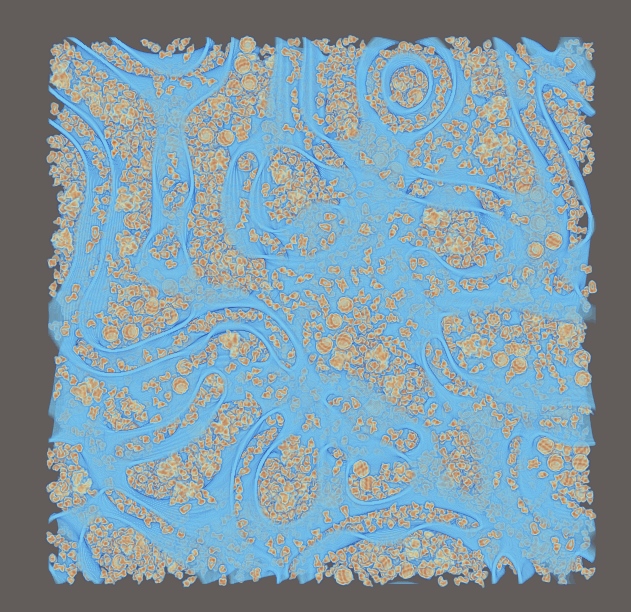
\includegraphics[width=0.5\textwidth]{archivos/sawlc-tomo.png}
     \caption{Tomograma generado con la inserción SAWCL.}
     \label{fig:sawcl-tomo}
\end{figure}

Este Trabajo Fin de Grado adapta e implementa \textbf{Tetris}~\cite{harastani2025template_repo}, un algoritmo de inserción de
proteínas basado en correlación cruzada 3D mediante FFT que, en cada paso, identifica
globalmente la posición óptima de colocación en lugar de muestrear candidatos al azar. El
algoritmo se adapta para operar en volúmenes que ya contienen estructuras biológicas
preexistentes (como membranas generadas por PolNet) y se extiende con un
mecanismo de crecimiento por clústeres guiado por semilla. Se desarrolla además una versión
acelerada por GPU con \textit{CuPy} que dirige automáticamente las operaciones más costosas
(correlación FFT 3D y muestreo global de semilla mediante \texttt{argwhere}) a la tarjeta
gráfica, manteniendo la misma lógica algorítmica que la versión
CPU. El trabajo se articula en un {repositorio independiente}~\cite{Hamo2025tetris_rep} cuyo objetivo es comparar Tetris
frente a SAWLC y evaluar si constituye un reemplazo viable para el módulo de inserción de
PolNet.\\

\begin{figure}[h]
     \centering
     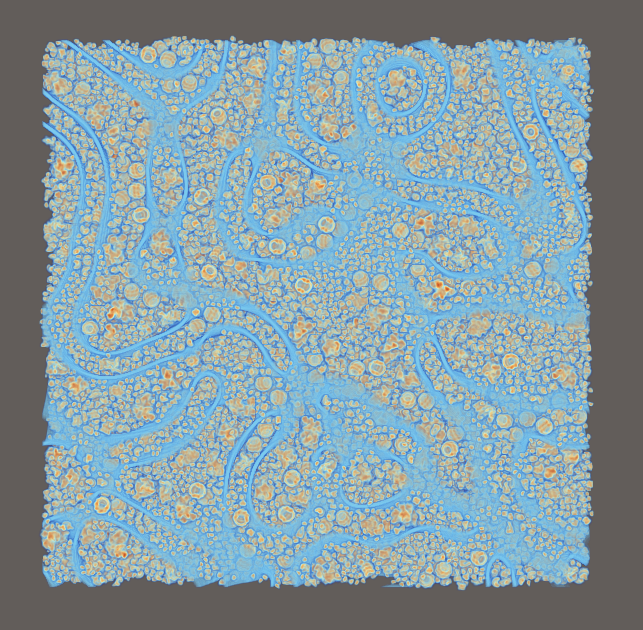
\includegraphics[width=0.5\textwidth]{archivos/tomo-tetris.png}
     \caption{Tomograma generado con la inserción Tetris.}
     \label{fig:sawcl-tomo}
\end{figure}

Los objetivos concretos del trabajo son: (i)~adaptar el algoritmo Tetris con correlación FFT
3D al contexto de PolNet, incorporando la información de membranas preexistentes y un
mecanismo de crecimiento por clústeres guiado por semilla; (ii)~desarrollar una versión
acelerada por GPU sobre \textit{CuPy} y rutas duales
CPU/GPU transparentes; (iii)~diseñar un banco de pruebas que compare ambos algoritmos en
ocupancia volumétrica, número de monómeros insertados y tiempo de ejecución; y
(iv)~analizar en qué escenarios Tetris supone una alternativa competitiva a SAWLC.\\

El resto del documento se organiza como sigue. El Capítulo~2 revisa el estado del arte:
fundamentos de la adquisición cryo-ET, métodos de generación de datos sintéticos y el
funcionamiento de SAWLC en el contexto de PolNet. El Capítulo~3 recoge el análisis de
requisitos. El Capítulo~4 describe el diseño e implementación de Tetris y del banco de
pruebas. El Capítulo~5 presenta y discute los resultados experimentales. El Capítulo~6 cierra
con las conclusiones y las líneas de trabajo futuro.

	%%%%%%%%%%%%%%%%%%%%%%%%%%%%%%%%%%%%%%%%%%%%%%%%%%%%%%%%%%%%%%%%%%%%%%%%
% Plantilla TFG/TFM
% Universidad de Murcia. Facultad de Informática
% Realizado por: José Manuel Requena Plens
% Modificado: Pablo José Rocamora Zamora
% Contacto: pablojoserocamora@gmail.com
%%%%%%%%%%%%%%%%%%%%%%%%%%%%%%%%%%%%%%%%%%%%%%%%%%%%%%%%%%%%%%%%%%%%%%%%


\chapter{Estado del arte}

\section{Contexto: Criomicroscopía Electrónica de Tomografía (Cryo-ET)}
La Criomicroscopía Electrónica de Tomografía (Cryo-ET) se ha consolidado como la técnica diagnóstica por excelencia para la observación de macromoléculas biológicas en su estado nativo. A diferencia de la cristalografía de rayos X, esta técnica permite visualizar el interior celular sin necesidad de cristalización o purificación previa de las muestras.

\subsection{Fundamentos y adquisición de datos}
El origen de la microscopía electrónica de transmisión (TEM) se remonta a 1931, con el desarrollo del primer prototipo por Max Knoll y Ernst Ruska, hito que le valdría a este último el Premio Nobel de Física en 1986. Sin embargo, la aplicación de esta técnica a muestras biológicas enfrentó inicialmente un obstáculo crítico: el daño por radiación. El haz de electrones de alta energía necesario para la obtención de imágenes provoca procesos de excitación molecular e ionización que destruyen las delicadas estructuras orgánicas\footnote{Esto se debe al bajo número atómico de los elementos que componen la materia orgánica (principalmente hidrógeno, carbono y oxígeno, etc.), los cuales presentan una alta sensibilidad a la radiólisis y un bajo contraste intrínseco bajo el haz de electrones.}. No fue hasta la década de 1980 cuando el desarrollo de métodos de vitrificación por Jacques Dubochet permitió preservar las muestras en condiciones nativas, contribución que le valió el Premio Nobel de Química en 2017, compartido con Joachim Frank y Richard Henderson por sus avances en la criomicroscopía electrónica.\\

La vitrificación es la piedra angular de la criomicroscopía moderna. Este proceso consiste en la congelación ultrarrápida de la muestra biológica, generalmente mediante su inmersión en etano líquido a temperaturas criogénicas. La velocidad del enfriamiento impide que las moléculas de agua se organicen en una estructura cristalina hexagonal, la cual expandiría su volumen y rompería las membranas celulares y complejos proteicos. En su lugar, el agua alcanza un estado sólido amorfo o vítreo, actuando como un soporte transparente a los electrones que inmoviliza y protege la estructura tridimensional de las macromoléculas.\\

A diferencia de la criomicroscopía electrónica convencional (cryo-EM), que suele centrarse en el análisis \textit{in vitro} de partículas purificadas, la Criomicroscopía Electrónica de Tomografía (cryo-ET) permite el estudio de las muestras \textit{in situ}. Esto significa que es posible visualizar macromoléculas como complejos proteicos, filamentos y membranas biológicas dentro de su contexto celular original y a una resolución sub-nanométrica.\\

La adquisición de datos en cryo-ET se basa en la generación de una \textbf{serie de inclinación} (\textit{tilt-series}). Dado que el microscopio produce proyecciones bidimensionales (2D) de la densidad electrónica, es necesario rotar la muestra de forma incremental —típicamente de $1^\circ$ en $1^\circ$ o de $2^\circ$ en $2^\circ$— dentro de un rango limitado, que habitualmente oscila entre los $-60^\circ$ y $+60^\circ$. Este rango se ve restringido por limitaciones mecánicas del portaobjetos y por el incremento del grosor efectivo que el haz de electrones debe atravesar en ángulos extremos, lo que reduce drásticamente la transmisión de señal.

\begin{figure}[H]
    \centering
    \includegraphics[width=0.8\textwidth]{archivos/haz.png}
    \caption{La cryo-ET consiste en capturar proyecciones mediante la inclinación de la muestra ($\pm60^{\circ}$) para su posterior reconstrucción en un tomograma tridimensional.}
    \label{fig:tilt-series}
\end{figure}

Finalmente, las proyecciones alineadas se procesan computacionalmente mediante algoritmos de reconstrucción matemática, siendo la Retroproyección Ponderada (\textit{Weighted Back-projection}, WBP) y los métodos iterativos como SIRT los más utilizados. El resultado es un \textbf{tomograma}: un volumen tridimensional compuesto por una rejilla de vóxeles que codifican la densidad electrónica local. Estos volúmenes se almacenan habitualmente en formato MRC, el cual permite gestionar grandes matrices de datos (por ejemplo, de $500\times500\times250$ vóxeles) y metadatos críticos como el tamaño de vóxel (típicamente 10\,\AA), parámetros fundamentales para la posterior inserción precisa de proteínas.


\subsection{Limitaciones: Ruido y el problema del Missing Wedge}

La Cryo-ET enfrenta desafíos físicos severos que condicionan de manera crítica la calidad, la resolución y la interpretación del volumen reconstruido. El primero de estos obstáculos es la \textbf{baja relación señal-ruido (SNR)}, una consecuencia directa de la extrema sensibilidad de las muestras biológicas al daño por radiación ionizante. Debido a que dosis elevadas de electrones provocarían la degradación estructural de la muestra y la rotura de enlaces químicos (radiólisis), la dosis acumulada durante toda la serie de inclinación debe mantenerse en niveles mínimos. Esto resulta en tomogramas con un contraste muy pobre donde las densidades electrónicas de las macromoléculas suelen quedar sepultadas bajo un ruido estocástico dominante, dificultando enormemente tanto la identificación visual por expertos como la eficacia de algoritmos de segmentación convencionales.\\

El segundo gran desafío técnico es el fenómeno denominado \textbf{Missing Wedge}. Debido a restricciones mecánicas del portaobjetos dentro de la columna del microscopio y al incremento exponencial del grosor efectivo de la muestra en ángulos extremos ($d/\cos \theta$), no es posible capturar proyecciones en el rango completo de $180^\circ$, limitándose habitualmente a un arco de $\pm60^\circ$. En el espacio de Fourier, esta falta de datos se traduce en una región con forma de cuña sin muestrear, lo que impide una reconstrucción isotrópica de la muestra. El efecto visual resultante es una distorsión geométrica característica: las estructuras aparecen significativamente elongadas en el eje vertical ($Z$) y las membranas u orgánulos orientados paralelamente al haz de electrones presentan una pérdida de resolución tan severa que pueden llegar a ser invisibles en el tomograma final.\\

\begin{figure}[H]
    \centering
    \includegraphics[width=0.7\textwidth]{archivos/missingWedge.png}
    \caption{Esquema de adquisición y espacio de Fourier con la cuña faltante (MW) y cuñas secundarias (BMW) que limitan la resolución vertical del tomograma.}
    \label{fig:missingWedge}
\end{figure}

Estos factores —el ruido masivo y las distorsiones del Missing Wedge— introducen artefactos y borrosidad direccional que comprometen la fidelidad de la información biológica capturada. Esta degradación intrínseca de los datos reales hace imprescindible el uso de simuladores avanzados para generar entornos sintéticos con un etiquetado conocido. Al disponer de volúmenes donde la posición, geometría y orientación de cada elemento están definidas con precisión absoluta, es posible entrenar redes neuronales profundas (CNNs) que aprendan a reconocer patrones complejos, compensar las anisotropías geométricas y extraer señales coherentes en tomogramas reales altamente degradados.

\section{Simulación de tomogramas mediante PolNet}
La generación de datos sintéticos se ha consolidado como una estrategia fundamental para mitigar las limitaciones intrínsecas al análisis de tomogramas reales. Mediante el uso de herramientas de simulación, es posible recrear digitalmente el entorno celular y emular los efectos ópticos del microscopio, produciendo volúmenes tridimensionales donde existe un control exhaustivo sobre las variables biológicas y los parámetros de degradación computacional.

\subsection{Datos sintéticos}
El motivo principal por el cual se evita el uso de datos experimentales reales como base exclusiva de entrenamiento para algoritmos de segmentación radica en las severas deficiencias inherentes a estas muestras. En Cryo-ET, una imagen real no constituye una representación fiel de la estructura biológica, sino una señal extremadamente degradada por el ruido y los condicionantes físicos del microscopio. Factores como la baja relación señal-ruido (SNR) y el artefacto del \textit{Missing Wedge} generan un entorno donde la frontera entre la estructura de interés y el ruido de fondo resulta difusa y ambigua.\\

Por tanto, el empleo de entornos simulados resulta fundamental por los siguientes factores críticos:

\begin{itemize}
    \item \textbf{Obtención de un \textit{Ground Truth} determinista:} En tomogramas reales, la anotación manual es un proceso extremadamente lento, costoso y propenso a errores. Al no existir una visualización clara, la segmentación depende de interpretaciones subjetivas que introducen sesgos; si el modelo se entrena con estas imprecisiones, el algoritmo heredará dichos errores. Por el contrario, los conjuntos de datos sintéticos permiten definir explícitamente la posición, orientación y geometría de cada estructura con precisión a nivel de vóxel. Esta ``verdad absoluta'' o etiquetado perfecto garantiza que el modelo aprenda sobre una base geométrica exacta.
    
    \item \textbf{Escalabilidad y eficiencia:} El entrenamiento robusto de redes neuronales profundas requiere miles de ejemplos etiquetados. Generar, vitrificar y anotar manualmente tal volumen de muestras reales es un proceso inasumible en términos de tiempo y recursos especializados. Los datos sintéticos permiten producir masivamente volúmenes etiquetados de forma automatizada y bajo condiciones controladas.

    \item \textbf{Aislamiento de variables y validación de robustez:} La simulación permite modelar de forma independiente fenómenos como el \textit{Missing Wedge} o diferentes niveles de SNR. Esta capacidad de parametrización es clave para evaluar la robustez y resiliencia de los modelos de segmentación ante degradaciones específicas, permitiendo optimizar el algoritmo antes de su aplicación en escenarios experimentales reales de alta complejidad.
\end{itemize}

\subsection{Arquitectura del framework PolNet}
PolNet es un framework de código abierto para la generación de tomodensigramas sintéticos de cryo-ET. Recibe especificaciones de estructuras biológicas como entrada y genera volúmenes 3D voxelizados con etiquetas como salida, proporcionando un conjunto de datos controlado y reproducible para el entrenamiento de modelos de aprendizaje profundo.

\subsubsection{Inputs}

Los inputs del framework son archivos de especificación que describen las estructuras biológicas a incluir:

\begin{itemize}
    \item \textbf{Membranas (.mbs)}: Definen la geometría de las membranas (por ejemplo, esferas, toroides o elipsoides) y su distribución general en el volumen. En la práctica, establecen el contexto estructural donde se ubicarán el resto de componentes biológicos.
    \item \textbf{Proteínas solubles (.pns)}: Especifican proteínas presentes en el citosol, es decir, no ancladas a membrana. Permiten controlar qué proteínas aparecen, su densidad aproximada y su organización espacial dentro del volumen.
    \item \textbf{Proteínas de membrana (.pms)}: Describen proteínas asociadas a superficies membranales. Son útiles para simular escenarios más realistas en los que ciertas macromoléculas se localizan preferentemente en membranas y no en el citosol libre.
    \item \textbf{Filamentos (.hns)}: Definen estructuras filamentosas como actina o microtúbulos, incorporando componentes del citoesqueleto. Su inclusión incrementa la complejidad estructural del tomograma y mejora el realismo del entorno celular.
    \item \textbf{Configuración (config.yaml)}: Reúne parámetros globales de generación, como tamaño del volumen, resolución (tamaño de voxel), número de tomogramas o semilla aleatoria. Estos valores determinan la escala del experimento y su reproducibilidad.
\end{itemize}

\subsubsection{Outputs}

El framework genera los siguientes archivos para cada tomograma:

\begin{itemize}
    \item \textbf{Volúmenes MRC}: Se generan principalmente dos volúmenes en formato estándar de cryo-ET: \texttt{tomo\_XXX\_den.mrc} (densidad electrónica simulada) y el mapa de etiquetas \texttt{tomo\_XXX\_lbl.mrc}. El primero se usa como entrada para tareas de análisis; el segundo como referencia para validación y entrenamiento supervisado.
    \item \textbf{Archivos de visualización (VTP)}: Incluyen representaciones geométricas de las estructuras insertadas, pensadas para inspección cualitativa y control visual de la generación. Son especialmente útiles para verificar si la distribución espacial de componentes es coherente con el escenario biológico deseado.
    \item \textbf{Tabla de mapeo (CSV)}: Relaciona cada tipo de estructura o archivo de entrada con sus etiquetas en el volumen. Facilita la trazabilidad entre configuración inicial y resultado final, algo clave para análisis cuantitativo y documentación experimental.
\end{itemize}

Estos outputs permiten entrenar modelos de segmentación automática y analizar la distribución de estructuras biológicas en el tomograma.

\subsection{Inserción de proteínas solubles a través del Self-Avoiding Worm-Like Chain (SAWLC)}

La inserción de proteínas solubles en PolNet se fundamenta en el modelo estocástico \textit{Self-Avoiding Worm-Like Chain} (SAWLC). Este algoritmo permite simular macromoléculas citosólicas como {cadenas poliméricas}\footnote{una cadena polimérica se entiende como un conjunto de monómeros conectados espacialmente.} discretas que mantienen una continuidad geométrica y evitan colisiones físicas mediante restricciones espaciales. A nivel computacional, el modelo SAWLC no realiza una simulación dinámica molecular, sino que actúa como un generador de configuraciones estocásticas basadas en el muestreo de posiciones y orientaciones plausibles.


\subsubsection{Fundamentos del modelo SAWLC}

SAWLC se emplea como un modelo generativo mesoscópico para construir configuraciones de proteínas solubles espacialmente plausibles bajo restricciones geométricas. El problema que se quiere resolver no es solo \textit{insertar proteínas}, sino insertarlas con una organización espacial realista e intentando llegar a un grado de ocupación alto. Una colocación uniforme o completamente aleatoria puede generar mapas de densidad poco realistas, con discontinuidades y patrones de empaquetamiento que no reflejan bien la estructura local del medio celular. Por este motivo, se utiliza SAWLC como estrategia intermedia entre dos extremos: la aleatoriedad sin restricciones y la simulación físico-molecular completa.\\

Formalmente, cada macromolécula $M_i$ del clúster se posiciona de forma aleatoria dentro de un conjunto de puntos candidatos $C_i$, definido por la intersección de una esfera de búsqueda y el volumen permitido:

\begin{equation}
C_i = S(x_{i-1}, d_i) \cap V
\end{equation}

Donde $x_{i-1}$ es la posición de la macromolécula anterior, $d_i$ es la distancia de enlace (\textit{link length}) y $S(x_{i-1}, d_i)$ representa una esfera centrada en $x_{i-1}$ con radio $d_i$. Esta operación se traduce en el código mediante un muestreo uniforme en una superficie esférica $S^2$:

\begin{equation}
x_i = x_{i-1} + t_i, \quad t_i \in S^2 \subset \mathbb{R}^3, \quad |t_i| = d_i
\end{equation}

Para asegurar una distribución estocástica de las orientaciones, cada monómero incorpora una rotación representada por un cuaternión unitario $q_i$ en el espacio $SO(3)$. La validez geométrica del paso $i$ está condicionada por una función de colisión $C(M_i, S)$, donde el monómero es aceptado si el solapamiento con el resto de la red y el volumen no supera la tolerancia $\epsilon$ permitida:

\begin{equation}
C(M_i, \text{VOI} \cup {M_1, \dots, M_{i-1}}) \leq \epsilon
\end{equation}

La ventaja principal de SAWLC es que impone continuidad geométrica y auto-evitación durante el crecimiento de cada cadena, lo que mejora el realismo estructural de los datos sintéticos sin perder control experimental. Además, el modelo soporta clústeres heterogéneos compuestos por $J$ tipos distintos de macromoléculas, permitiendo simular entornos citosólicos complejos. En términos prácticos, permite regular la densidad y longitud mediante parámetros explícitos, manteniendo la reproducibilidad mediante el uso de una semilla aleatoria. Por tanto, SAWLC se adopta aquí como un \textbf{modelo generativo orientado a la plausibilidad geométrica}: no pretende reproducir toda la dinámica biofísica de las proteínas, pero sí generar configuraciones suficientemente realistas y controlables para tareas de entrenamiento y validación de algoritmos de segmentación en criotomografía electrónica.

\begin{figure}[H]
    \centering
    \includegraphics[width=0.9\textwidth]{archivos/sawlc_schema.png}
    \caption{Esquema del algoritmo SAWLC: Muestreo de semilla, Crecimiento válido, Detección de colisión y Reintento/Finalización por congestión espacial.}
    \label{fig:sawlc-schema}
\end{figure}
 
\subsubsection{Parámetros del algoritmo}

Para describir el comportamiento del método y su control sobre la densidad y organización del clúster, los parámetros más relevantes definidos en la implementación de PolNet son:

\begin{itemize}
    \item $\rho^*$: Grado de ocupación objetivo, definido como el porcentaje del volumen del VOI que debe ser cubierto por las macromoléculas.
    \item $L_{max}$: Longitud máxima de la cadena, que limita el número de unidades estructurales (monómeros) por cada polímero generado.
    \item $d_i$: Distancia de enlace (\textit{link length}) entre monómeros consecutivos, que determina el radio de la esfera de muestreo $S(x_{i-1}, d_i)$.
    \item $T_c$: Número máximo de intentos para localizar una semilla inicial válida ($x_0$) dentro del volumen libre.
    \item $T_m$: Número máximo de intentos para proponer una extensión de la cadena ($x_i$) antes de dar por finalizado el crecimiento del polímero actual.
    \item $\epsilon$: Tolerancia de solapamiento (\textit{over\_tolerance}), definida como la fracción [0, 1] de puntos de la superficie del monómero permitidos dentro de otra estructura.
    \item $J$: Número de tipos distintos de macromoléculas ($M_j$) que pueden conformar un clúster heterogéneo.
    \item $v_{size}$: Tamaño del vóxel del volumen, parámetro crítico para la discretización de las mallas y la validación en el VOI.
\end{itemize}

\subsubsection{Pseudocódigo}

\begin{algorithm}[H]
    \caption{Inserción de proteínas solubles mediante SAWLC}
    \label{alg:sawlc_tecnico}
    \KwIn{VOI ($V$), Proteínas ($P$), $\rho^*, L_{max}, d_i, T_c, T_m, \epsilon, J, v_{size}$}
    \KwOut{Distribución final de polímeros y ocupación actualizada $\rho$}

    Inicializar estado del volumen y ocupación actual $\rho \gets 0$\;

    \While{$\rho < \rho^*$}{
        $intentos\_c \gets 0$\;
        \While{$intentos\_c < T_c$}{
            $x_0 \gets$ muestrear\_semilla\_válida($V, v_{size}$)\;
            \If{$x_0$ es válida}{
                $C \gets$ inicializar\_cadena($x_0, P_j$)\;
                \For{$i = 1 \dots L_{max}$}{
                    $intentos\_m \gets 0$\;
                    \While{$intentos\_m < T_m$}{
                        Proponer $x_i \in S(x_{i-1}, d_i) \cap V$\;
                        $q_i \gets$ gen\_cuaternion\_aleatorio()\;
                        \If{validar\_colision($M_i, \rho, \epsilon, v_{size}$)}{
                            Aceptar monómero e insertar en $C$\;
                            Actualizar ocupación $\rho$\;
                            \textbf{break}\;
                        }
                        $intentos\_m \gets intentos\_m + 1$\;
                    }
                    \If{$intentos\_m == T_m$ o $\rho \ge \rho^*$}{\textbf{break}\;}
                }
                \textbf{break} \tcp*{Cadena completada o detenida}
            }
            $intentos\_c \gets intentos\_c + 1$\;
        }
        \If{$intentos\_c == T_c$}{\textbf{break} \tcp*{Saturación del volumen}}
    }
    \Return Distribución de polímeros y $\rho$\;
\end{algorithm}

\subsubsection{Análisis de complejidad y orden de magnitud}

El coste computacional del algoritmo SAWLC no depende exclusivamente del número de proteínas finalmente insertadas, sino del volumen total de intentos, tanto exitosos como fallidos, necesarios para intentar alcanzar la ocupación objetivo $\rho^*$. Basándose en el flujo lógico de los bucles de control implementados, el coste teórico se expresa mediante la siguiente relación de complejidad:

\[
O(T_c \cdot L_{max} \cdot T_m \cdot C_{val})
\]

En esta expresión, el componente crítico es el factor de validación $C_{val}$, que representa el coste de verificar la ausencia de colisiones mediante {mallas de superficie}\footnote{En el contexto de PolNet, una malla de superficie (\textit{surface mesh}) es una representación discreta de la frontera exterior de una macromolécula mediante un objeto de tipo \texttt{vtkPolyData}.}. A diferencia de los parámetros de control definidos anteriormente, este coste es dinámico y depende de la resolución de la malla ($N_{puntos}$) y del número de objetos ya presentes en el volumen, lo que obliga al algoritmo a realizar comprobaciones geométricas más costosas conforme el sistema se densifica.

\paragraph{Comportamiento según el grado de ocupación}

El coste real presenta una fuerte dependencia no lineal con respecto a la ocupación actual $\rho$:

\begin{itemize}
    \item \textbf{Régimen de baja densidad ($\rho \ll \rho^*$):} La probabilidad de colisión es mínima, permitiendo que la mayoría de las propuestas se acepten en el primer intento. En esta fase, el comportamiento es cuasi-lineal respecto al número de monómeros insertados.
    \item \textbf{Régimen de congestión molecular (\textit{crowding}):} A medida que el espacio libre se fragmenta, la probabilidad de que una propuesta estocástica $x_i$ sea válida disminuye exponencialmente. En este escenario, el sistema agota sistemáticamente los umbrales de reintento $T_m$ y $T_c$.
\end{itemize}

Por tanto, el cuello de botella computacional de SAWLC reside en el procesamiento de los intentos fallidos, donde el sistema invierte recursos significativos en validaciones geométricas de candidatos que finalmente son rechazados por colisión.

\subsubsection{Limitaciones del modelo SAWLC}

Aunque el método SAWLC es eficaz para generar entornos macromoleculares con continuidad estructural, presenta restricciones técnicas intrínsecas que condicionan su rendimiento en escenarios de alta densidad:

\begin{itemize}
    \item \textbf{Dependencia multivariante y ajuste empírico:} El éxito de la simulación está sujeto a una interdependencia compleja entre parámetros como la tolerancia de solapamiento ($\epsilon$), la longitud de enlace ($d_i$) y los umbrales de reintento ($T_c, T_m$). La falta de un modelo analítico para predecir la convergencia obliga a un ajuste empírico laborioso para cada tipo de proteína y ocupación objetivo.
    
    \item \textbf{Saturación por fragmentación del espacio libre:} El algoritmo no garantiza alcanzar la ocupación máxima teórica ($\rho^*$). Debido a su naturaleza de crecimiento secuencial y "ciego", el sistema suele quedar atrapado en configuraciones donde el espacio libre remanente es inferior al volumen del monómero o está distribuido en huecos inconexos que no permiten la extensión de la cadena.
    
    \item \textbf{Barrera de {entropía}\footnote{No confundir con la entropía de Shannon. En polímeros, la entropía configuracional mide el número de estados espaciales accesibles para la cadena. La ``barrera'' surge cuando la falta de huecos libres reduce estos estados, provocando que la búsqueda estocástica ($T_m$) falle sistemáticamente por pura probabilidad.} en escenarios de \textit{crowding}:} A medida que el volumen se densifica, la probabilidad de que una propuesta de extensión $x_i$ sea válida tiende a cero de forma exponencial. Esto genera un incremento masivo en el número de validaciones geométricas fallidas, provocando que el algoritmo se detenga prematuramente al agotar los intentos $T_m$, dejando el tomograma con una ocupación real significativamente inferior a la biológica.
    
    \item \textbf{Inconsistencia en el empaquetamiento determinista:} Al ser un proceso estocástico basado en semillas aleatorias, la organización local del clúster es altamente variable. Esta falta de control sobre la disposición espacial fina dificulta la simulación realistas.
\end{itemize}

En consecuencia, el modelo SAWLC debe entenderse como un procedimiento generativo orientado a la verosimilitud estructural más que a la eficiencia de empaquetamiento. Esta limitación computacional para obtener entornos de alta densidad molecular justifica la exploración de nuevos algoritmos que gestionen el espacio de forma determinista para maximizar la ocupación del volumen.

\section{Algoritmo Tetris: Inserción de alta densidad}

Para superar las limitaciones de empaquetamiento y alcanzar un mayor grado de ocupancia, surge el algoritmo \textbf{Tetris}, una técnica de gestión espacial para generar muestras tridimensionales con una alta congestión molecular (\textit{crowding}). A diferencia de los métodos de crecimiento polimérico, este algoritmo permite posicionar las proteínas de forma compacta y eficiente.

\subsection{Fundamentos del modelo Tetris}

El algoritmo Tetris opera bajo un principio intuitivo de optimización de proximidad: coloca las moléculas iterativamente, posicionando cada nueva unidad en la ubicación más cercana posible a las ya existentes sin producir colisiones. El proceso se basa en el procesamiento de volúmenes binarizados y el uso de operadores de correlación para identificar el espacio disponible.\\

El núcleo del algoritmo reside en la creación de una \textbf{cáscara de inserción} ($in\text{-}shell$). Para cada molécula candidata $M$, se genera una versión binarizada y dilatada; al restar la versión binarizada de la dilatada, se obtiene un margen espacial que define la distancia mínima permitida respecto a otros objetos. Matemáticamente, esta guía espacial $I$ se define como:

\begin{equation}
I = \text{dilate}(\text{bin}(M), r) - (\text{bin}(M) \cdot \infty)
\end{equation}

Donde $\text{bin}(\cdot)$ es el operador de binarización, $r$ es el radio del elemento estructural de dilatación y el factor infinito asegura que el núcleo de la molécula sea una zona de colisión prohibida. La posición óptima se determina mediante la correlación ($\star$) de esta cáscara con el volumen acumulado del tomograma ($O$), generando un mapa de correlación ($c\text{-}map$) $C$:

\begin{equation}
C = I \star \text{bin}(O)
\end{equation}

Los valores positivos en este mapa indican posiciones viables, y el algoritmo selecciona sistemáticamente el índice del valor máximo $x_{opt}$ para garantizar la máxima compacidad:

\begin{equation}
x_{opt} = argmax(C)
\end{equation}

A partir de la dinámica ilustrada en la Figura \ref{fig:tetris}, el funcionamiento detallado del algoritmo se desglosa en las siguientes etapas críticas:

\begin{itemize}
    \item \textbf{Selección y rotación estocástica}: El proceso se inicia extrayendo una molécula de la base de datos de entrada (ya sea una plantilla objetivo o un distractor) y aplicándole una rotación aleatoria uniforme para asegurar que el empaquetamiento final sea isotrópico y no presente sesgos de orientación.
    
    \item \textbf{Tratamiento del primer ejemplar}: En la primera iteración, el objeto se sitúa automáticamente en el centro de un volumen vacío expandido, estableciendo el núcleo inicial del clúster o \textit{current output}.
    
    \item \textbf{Preprocesamiento y binarización}: Para las moléculas sucesivas, el sistema realiza un suavizado (\textit{smooth}) mediante filtros de paso bajo y una binarización. Este paso es fundamental para transformar la densidad electrónica compleja en una máscara geométrica de ocupación binaria.
    
    \item \textbf{Generación de la \textit{in-shell}}: La versión binarizada del nuevo objeto se dilata según un radio de seguridad definido por el usuario. Al restar la máscara binarizada original (multiplicada por un valor de peso infinito) de la versión dilatada, se genera la \textbf{\textit{in-shell}}. Esta estructura actúa como una guía que delimita la zona de contacto permitida: define dónde puede estar el centro de la nueva molécula para que su borde toque a las ya existentes sin llegar a solaparlas.
    
    \item \textbf{Análisis de viabilidad mediante el \textit{C-map}}: Se ejecuta una operación de correlación entre la \textit{in-shell} y la versión binarizada del volumen acumulado actual. El resultado es el mapa de correlación o \textbf{\textit{C-map}}, donde los valores positivos representan coordenadas de inserción válidas y los valores negativos o nulos representan posiciones de colisión o excesivamente alejadas.
    
    \item \textbf{Optimización de la compacidad}: El algoritmo identifica el índice que contiene el \textbf{valor máximo absoluto} dentro del \textit{C-map}. Al elegir este máximo, se garantiza que la molécula se inserte en la posición más cercana posible al clúster existente, logrando la máxima densidad molecular (\textit{highest compactness}).
    
    \item \textbf{Saturación y fin del proceso}: El ciclo continúa actualizando la salida (\textit{update output}) hasta que el \textit{C-map} resultante es completamente negativo. Esto indica que el espacio libre se ha fragmentado hasta tal punto que no es posible insertar más proteínas bajo las restricciones impuestas, marcando el fin de la simulación por saturación.
\end{itemize}

\begin{figure}[H]
    \centering
    \includegraphics[width=0.9\textwidth]{archivos/tetris.jpeg}
    \caption{Esquema del algoritmo Tetris: se aplica un suavizado, binarizado, dilatación, subtración, correlación y posterior comprobación en el mapa de correlación.}
    \label{fig:tetris}
\end{figure}

\subsection{Parámetros del algoritmo}

Basado en la metodología de \textit{Template Learning}, el control del empaquetamiento y la calidad de la discretización depende de los siguientes parámetros:

\begin{itemize}
    \item \textbf{Radio del elemento estructural ($r$):} Define el grado de dilatación de la molécula y, por tanto, controla directamente la distancia mínima entre proteínas y la compacidad final de la muestra.
    \item \textbf{Desviación estándar ($\sigma$):} Parámetro del filtro gaussiano de paso bajo aplicado antes de la binarización para suavizar las densidades.
    \item \textbf{Umbral de volumen ($v_{th}$):} Valor utilizado para la binarización de los mapas de densidad.
    \item \textbf{Frecuencia de tipos ($f$):} Ratio que determina la proporción entre proteínas objetivo (\textit{templates}) y moléculas de distracción (\textit{distractors}) para mantener un equilibrio de densidad volumétrica.
\end{itemize}

\subsection{Pseudocódigo}

\begin{algorithm}[H]
    \caption{Generación de volúmenes congestionados mediante Tetris}
    \label{alg:tetris_tecnico}
    \KwIn{Proteínas PDB ($P$), Distractor moleculas ($D$), Volumen ($V$), $r, \sigma, v_{th}$}
    \KwOut{Volumen 3D y coordenadas orientadas}
    Seleccionar molécula inicial $M_0$ y posicionar en el centro de $V$\;
    Actualizar salida actual $O \gets M_0$\;
    
    \While{Existan posiciones válidas}{
        Seleccionar nueva molécula $M_i \in \{P \cup D\}$ y aplicar rotación aleatoria uniforme\;
        $M_{bin} \gets$ suavizar\_y\_binarizar($M_i, \sigma, v_{th}$)\;
        $M_{dil} \gets$ dilatar($M_{bin}, r$)\;
        $In\_shell \gets M_{dil} - (M_{bin} \cdot \infty)$ \tcp*{Generar guía espacial}
        
        $C\_map \gets$ correlacionar($In\_shell$, binarizar($O$))\;
        
        \If{$C\_map$ tiene valores positivos}{
            $pos\_max \gets$ índice del valor máximo en $C\_map$\;
            Insertar $M_i$ en $O$ en la posición $pos\_max$\;
            Actualizar volumen de salida $O$\;
        }
        \Else{
            \textbf{break} \tcp*{Saturación alcanzada: no hay más huecos}
        }
    }
    \Return Volumen $O$ y registro de coordenadas\;
\end{algorithm}

\subsection{Análisis de complejidad y justificación}

A diferencia de los enfoques estocásticos utilizados en SAWLC, el algoritmo Tetris presenta una arquitectura optimizada para la gestión de volúmenes discretos mediante un proceso determinista. Para la inserción de $N$ proteinas solubles en un tomograma de $V$ vóxeles, el coste computacional se rige por la operación de correlación necesaria en cada iteración, expresándose formalmente como:

\begin{equation}
O(N \cdot V \log V)
\end{equation}

Esta complejidad se fundamenta en el empleo de la Transformada Rápida de Fourier (FFT) para el cálculo del mapa de correlación ($c\text{-}map$), permitiendo que el procesamiento escale de forma eficiente con las dimensiones del volumen. Al buscar sistemáticamente el máximo global de probabilidad de inserción, el diseño del algoritmo permite evitar el estancamiento configuracional característico de los métodos basados en muestreos aleatorios.\\

La justificación técnica de esta metodología sobre SAWLC reside en su capacidad para modelar el \textbf{empaquetamiento molecular} (\textit{molecular crowding}) con geometrías genéricas no esféricas de forma sistemática. Mientras que el crecimiento de cadenas aleatorias puede verse interrumpido prematuramente por la fragmentación del espacio libre, el algoritmo Tetris garantiza un llenado determinista de los intersticios, eliminando espacios vacíos no estructurados y permitiendo alcanzar densidades biológicamente verosímiles para el entrenamiento de modelos de \textit{deep learning}.\\

En el contexto de su integración en el \textit{framework} \textbf{PolNet}, se hace evidente que el algoritmo debe ser adaptado para adquirir consciencia del contexto estructural previo. Bajo esta premisa, la máscara de ocupación inicial debe incorporar el volumen de las densidades preexistentes, como membranas y filamentos, garantizando que el mapa de correlación identifique posiciones válidas que respeten estrictamente los demás elementos biológicos. Asimismo, se requiere el diseño de un mecanismo de generación de clústeres inteligente que trascienda la dispersión aleatoria; para ello, el algoritmo debe utilizar las posiciones de máxima afinidad geométrica para nuclear el crecimiento de las proteínas solubles, asegurando una ocupación homogénea y compacta de la totalidad del volumen del tomograma.



	%%%%%%%%%%%%%%%%%%%%%%%%%%%%%%%%%%%%%%%%%%%%%%%%%%%%%%%%%%%%%%%%%%%%%%%%
% Plantilla TFG/TFM
% Universidad de Murcia. Facultad de Informática
% Realizado por: José Manuel Requena Plens
% Modificado: Pablo José Rocamora Zamora
% Contacto: pablojoserocamora@gmail.com
%%%%%%%%%%%%%%%%%%%%%%%%%%%%%%%%%%%%%%%%%%%%%%%%%%%%%%%%%%%%%%%%%%%%%%%%


\chapter{Análisis de objetivos y metodología}

\section{Objetivos}
El objetivo general de este proyecto es optimizar y acelerar el proceso de generación de tomogramas sintéticos para el \textit{framework} \textbf{PolNet}. Específicamente, se busca perfeccionar la inserción de proteínas solubles en entornos biológicos complejos que contienen estructuras preexistentes, como membranas, logrando una alta densidad en la muestra. Para alcanzar esta meta, se han definido los siguientes objetivos específicos:

\begin{itemize}
     \item \textbf{Estudio comparativo de la capacidad de empaquetamiento}: Evaluar el grado de ocupación (\textit{occupancy}) alcanzado por el algoritmo \textbf{Tetris} frente al modelo \textbf{SAWLC}. Se analizará el tiempo de ejecucción, el grado de ocupancia, el número de proteínas insertadas, etc.
    
    \item \textbf{Adaptación del algoritmo Tetris}: Modificar el proceso de inserción del algoritmo Tetris\footnote{El algoritmo por defecto no tiene en cuenta los elementos biológicos preexistentes antes del proceso de inserción de proteínas.} original para que sea capaz de reconocer el volumen ocupado por elementos biológicos preinsertados en \textbf{PolNet}. Esto implica que la máscara de ocupación inicial debe integrar las densidades de membranas para que el mapa de correlación (\textit{c-map}) identifique únicamente posiciones biológicamente válidas.
    
   \item \textbf{Generación inteligente de clústeres}: Desarrollar un mecanismo de crecimiento local guiado por correlación para favorecer agrupaciones compactas, reduciendo la dispersión aleatoria y los intentos fallidos.
    
    \item \textbf{Aceleración del proceso mediante computación en GPU}: Diseñar y ejecutar una versión del algoritmo optimizada para su procesamiento paralelo en tarjeta gráfica. El objetivo es aprovechar la eficiencia de la GPU en operaciones de correlación y Transformadas Rápidas de Fourier (FFT) para reducir drásticamente los tiempos de simulación.
    
    \item \textbf{Validación del modelo (\textit{Ground Truth})}. Verificar el grado de ocupancia y coherencia geométrica de los tomogramas generados, evaluando su adecuación como datos de entrenamiento para tareas de detección de partículas (\textit{particle picking}) mediante modelos de \textit{Deep Learning}.
\end{itemize}


\section{Metodología}

La metodología seguida en este proyecto se estructura en cinco fases secuenciales que abarcan desde la configuración del entorno de trabajo hasta la validación experimental del sistema desarrollado.

\subsection{Fase 1: Creación del entorno}

El primer paso para garantizar la validez y la reproducibilidad de los resultados obtenidos en este trabajo consiste en la definición y configuración de un entorno de ejecución robusto. Dado que el procesamiento de tomogramas y la simulación de densidades proteicas requieren una alta capacidad computacional, es fundamental detallar tanto la arquitectura física (hardware) como el ecosistema de software y dependencias utilizado.
\begin{enumerate}
    \item \textbf{Sistema usado:} Todas las pruebas, ejecuciones y benchmarks de este proyecto se realizaron en una estación de trabajo de escritorio en el laboratorio AIKE con las siguientes especificaciones:

        \begin{itemize}
            \item \textbf{CPU}: AMD Ryzen 9 5900X
            \begin{itemize}
                \item 12 núcleos / 24 hilos
                \item Frecuencia base: 3.7 GHz; frecuencia turbo máxima: 4.8 GHz
            \end{itemize}
            \item \textbf{GPU}: NVIDIA RTX 4090 (24 GB GDDR6X)
            \item \textbf{RAM}: 64 GB DDR4
            \item \textbf{Almacenamiento}: SSD NVMe Samsung 980 PRO (1 TB) y HDD Seagate IronWolf 12 TB (ST12000VN0008).
            \item \textbf{Sistema operativo}: Ubuntu 24.04.3 LTS.
            \item \textbf{Driver de NVIDIA}:  Versión 580.126.09. 
            \item \textbf{Versión de CUDA Toolkit:} 12.0 
        \end{itemize}

    \item \textbf{Entorno virtual: } El desarrollo y la ejecución del código se llevaron a cabo dentro de un entorno virtual de Python (\texttt{venv}), garantizando el aislamiento de dependencias respecto al sistema y la reproducibilidad de los experimentos. El repositorio incluye el script \texttt{setup\_env.sh} (Linux/Mac) que automatiza la creación del entorno, detecta si hay GPU disponible e instala las dependencias correspondientes:

    \begin{lstlisting}[language=bash]
    bash setup_env.sh
    source .venv/bin/activate
    \end{lstlisting}

    Las dependencias del proyecto se dividen según el tipo de ejecución:
    
    \begin{table}[H]
        \centering
        \begin{tabular}{|l|c|l|}
        \hline
        \textbf{Librería} & \textbf{Versión mínima} & \textbf{Propósito} \\
        \hline
        \texttt{numpy} & $\geq$ 2.0 & Operaciones con arrays multidimensionales \\
        \texttt{scipy} & $\geq$ 1.10 & Filtros, correlaciones FFT y morfología \\
        \texttt{scikit-image} & $\geq$ 0.20 & Procesamiento de imágenes y morfología 3D \\
        \texttt{mrcfile} & $\geq$ 1.4 & Lectura/escritura de archivos MRC \\
        \texttt{vtk} & $\geq$ 9.2 & Visualización 3D y exportación VTP \\
        \texttt{pandas} & $\geq$ 2.0 & Análisis y procesamiento de métricas \\
        \texttt{imageio} & $\geq$ 2.31 & Generación de animaciones y GIFs \\
        \hline
        \multicolumn{3}{|c|}{\textit{Exclusivas del entorno GPU (CUDA 12)}} \\
        \hline
        \texttt{matplotlib} & $\geq$ 3.7 & Generación de gráficas comparativas \\
        \texttt{cupy-cuda12x} & $\geq$ 14.0 & Operaciones GPU equivalentes a NumPy/SciPy \\
        \texttt{pyfftw} & $\geq$ 0.13 & Transformadas de Fourier optimizadas en CPU \\
        \hline
        \end{tabular}
        \caption{Dependencias del proyecto por tipo de entorno.}
        \label{tab:dependencias}
    \end{table}
     El código fuente se organiza en tres módulos: \texttt{sawlc/}, que contiene \texttt{PolNet} integrado directamente desde su código fuente al emplearse una versión modificada; \texttt{tetris\_3d/}, el módulo principal con el algoritmo Tetris sobre tomogramas 3D; y \texttt{tetris\_2d/}, una versión en dos dimensiones usada para validación conceptual. Ambos algoritmos producen ficheros \textbf{MRC}: Tetris genera \texttt{tomo\{idx\}\_den\{n\}.mrc} (tomograma sintético) y \texttt{tomo\{idx\}\_lbl\{n\}.mrc} (etiquetas: \texttt{0}=vacío, \texttt{1}=membrana, \texttt{2}=proteína); SAWLC produce ficheros equivalentes más archivos \textbf{VTP} con la representación poligonal de las estructuras. Para la inspección visual se emplearon \textbf{ParaView} y \textbf{3dmod} (suite IMOD).

    \end{enumerate}

\subsection{Fase 2: Análisis y Estudio del algoritmo Tetris}

El punto de partida del trabajo consistió en la comprensión profunda del algoritmo Tetris descrito en el artículo \textit{Template Learning} \cite{harastani2025template}. Esta fase incluyó:

\begin{enumerate}
    \item \textbf{Estudio del código de referencia}: Análisis de la implementación original para identificar las operaciones críticas y costosas del algoritmo como la rotación aleatoria de moléculas, binarización mediante filtrado gaussiano, generación de la \textit{in-shell} por dilatación morfológica, correlación FFT y selección del máximo del \textit{c-map}. La complejidad global del algoritmo, tal y como se justifica en la Sección del estado del arte (véase análisis de complejidad de Tetris), es:
    \begin{equation}
        O(N \cdot V \log V)
    \end{equation}
    donde $N$ es el número de proteínas insertadas y $V$ el número de vóxeles del tomograma. 

    \item \textbf{Identificación de las operaciones computacionalmente costosas}: A partir de la complejidad teórica $O(N \cdot V \log V)$, se identifican dos operaciones candidatas a ser cuello de botella: la correlación FFT 3D, cuyo coste es $O(V \log V)$ por inserción y domina cuando el volumen $V$ es grande, y el muestreo de posición válida (\texttt{pick\_seed}), una nueva funcionalidad introducida en este trabajo, con coste lineal $O(V)$ por llamada. Las operaciones de rotación afín y generación de \textit{in-shell} tienen un coste proporcional al tamaño de la caja de la proteína —mucho menor que $V$— y son teóricamente despreciables. La medición empírica de estos tiempos sobre la implementación adaptada se presenta en la Fase~3 (Punto~6), una vez descritas todas las modificaciones sobre las que se aplica el perfilado.

    \item \textbf{Verificación de la lógica del algoritmo}: Comprobación de que el principio de inserción secuencial por máxima proximidad (selección del $\arg\max(C)$ del mapa de correlación) garantiza el empaquetamiento compacto sin solapamientos gracias a la penalización negativa en el núcleo de la \textit{in-shell}. La condición de terminación —\textit{c-map} completamente negativo— implica que no existe ninguna posición biológicamente válida donde insertar la próxima proteína, lo que marca la saturación del volumen. La Figura~\ref{fig:tomo-occupancy} muestra un tomograma vacío generado con la proteína \textit{2uv8\_10A.pns} en un volumen vacío de $500\times500\times250$ vóxeles, alcanzando un grado de ocupancia del 32\% con 2\,552 monómeros insertados.

    \begin{figure}[H]
        \centering
        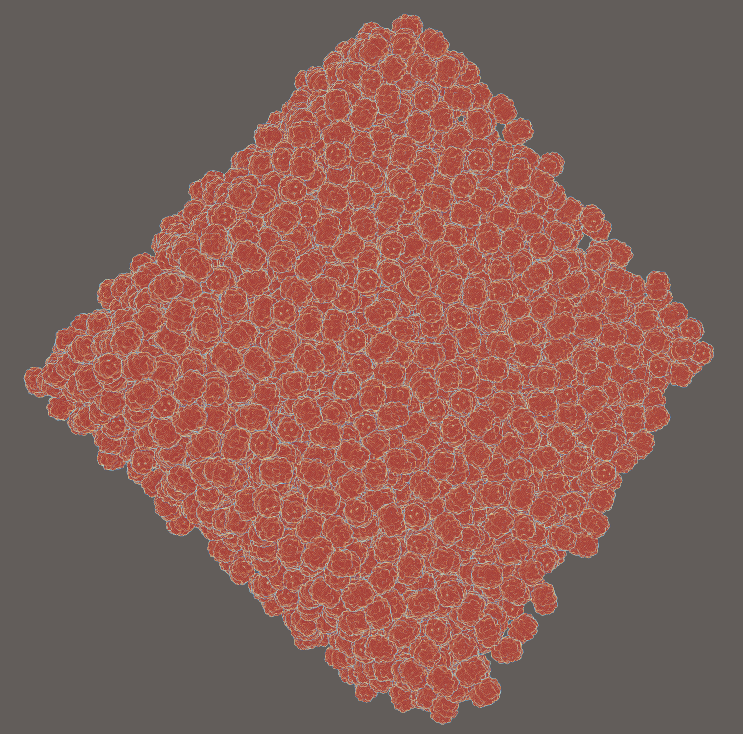
\includegraphics[width=0.5\textwidth]{archivos/tomo_occupany_breakdown.png}
        \caption{Tomograma sintético generado con la proteína \textit{2uv8\_10A.pns} en un volumen de $500\times500\times250$ vóxeles. Se alcanzó un grado de ocupancia del 32\% con 2\,552 monómeros insertados.}
        \label{fig:tomo-occupancy}
    \end{figure}
\end{enumerate}

\subsection{Fase 3: Implementación y Adaptación en PolNet}

Esta fase se centró en adaptar el algoritmo Tetris al \textit{framework} PolNet con el objetivo de facilitar una futura integración. En particular, fue necesario modificar el algoritmo para que tuviera en cuenta estructuras biológicas preexistentes, como membranas, durante el proceso de inserción de proteínas solubles y añadir una generación de clústeres inteligente.

\begin{enumerate}

     \item \textbf{Integración de elementos biológicos previo}: El algoritmo original asume un volumen inicialmente vacío; inicializa su \textit{output volume} a cero y empieza a insertar proteínas sin conocimiento de ninguna estructura preexistente. Para permitir la inserción de proteínas sobre membranas ya generadas por PolNet, se añadió una etapa de pre-carga que escribe las densidades de los elementos preexistentes directamente en el volumen de salida del algoritmo antes de comenzar la inserción:

    \begin{algorithm}[H]
        \caption{Pre-carga de membrana en el volumen Tetris}
        \label{alg:preload}
        \KwIn{Volumen MRC de membrana ($V_{mem}$), umbral proteico $\theta$}
        \KwOut{\textit{output\_volume} inicializado con regiones prohibidas}
        $allowed\_mask \gets \lnot(V_{mem} > 0)$ \tcp*{True = vóxel libre}
        $tetris.output\_volume \gets \mathbf{0}$ \tcp*{inicialización original}
        $tetris.output\_volume[\lnot allowed\_mask] \gets \infty$ \tcp*{nueva etapa: $\rho_{mem} \gg \theta$}
    \end{algorithm}

    Al asignar $\rho_{membrane} = 500.0 \gg \theta_{protein}$ a todos los vóxeles de membrana, estos son detectados como «ocupados» por el mecanismo de colisión del algoritmo en todas las iteraciones posteriores, sin necesidad de modificar la lógica interna de inserción. Adicionalmente, la \textit{allowed\_mask} binaria se propaga a la función de correlación para penalizar con $-10^9$ cualquier candidato de inserción que caiga sobre un vóxel de membrana. Esto garantiza que la inserción de proteínas solubles se limite a regiones biológicamente permitidas, independientemente de la intensidad local de la correlación.

    \item \textbf{Sistema de semillas inteligente y generación de clústeres}: El algoritmo original coloca la primera molécula en el centro del volumen y luego crece por proximidad, dejando los bordes del tomograma vacíos y sin tener en cuenta otros elementos. Se desarrolló una función \texttt{pick\_seed()} que muestrea uniformemente posiciones válidas en todo el espacio libre viable:
    \begin{equation}
    \text{viable}[z, y, x] = \text{allowed}[z, y, x] \land (\text{output}[z, y, x] \leq \theta) \land (z, y, x \notin \text{border})
    \end{equation}

    donde $\text{border}$ denota la región de margen ($\lfloor box\_size/2 \rfloor$ vóxeles desde cada borde), garantizando que la proteína quepa íntegra. Su funcionamiento se detalla en el Algoritmo~\ref{alg:pick_seed}:

    \begin{algorithm}[H]
        \caption{\texttt{pick\_seed}: muestreo uniforme de semilla válida}
        \label{alg:pick_seed}
        \KwIn{$allowed\_mask$, $output\_volume$, umbral $\theta$, $box\_size$}
        \KwOut{Coordenada semilla $(z,y,x)$ o $\varnothing$}
        $half \gets \lfloor box\_size / 2 \rfloor$\;
        $empty \gets allowed\_mask \land (output\_volume \leq \theta)$\;
        $viable \gets \{(z,y,x) \in empty : half \leq z < D_z{-}half,\; half \leq y < D_y{-}half,\; half \leq x < D_x{-}half\}$\;
        \If{$viable = \varnothing$}{\Return $\varnothing$}
        \Return coordenada aleatoria uniforme de $viable$\;
    \end{algorithm}

    El mecanismo de crecimiento de clústeres combina \texttt{pick\_seed()} con un contador de fallos consecutivos controlado por el parámetro  \texttt{$T_{cluster}$} (fijado a 10). El Algoritmo~\ref{alg:cluster} describe el bucle de inserción para cada tipo de proteína:

    \begin{algorithm}[H]
        \caption{Crecimiento de clúster guiado por semilla}
        \label{alg:cluster}
        \KwIn{$allowed\_mask$, $output\_volume$, proteína $M$, $\theta$, $T_{cluster} = 10$}
        \KwOut{Proteínas insertadas en el volumen}
        $target \gets \texttt{pick\_seed}(allowed\_mask, output, \theta, box\_size)$\;
        $failures \gets 0$\;
        \While{$failures < T_{cluster}$}{
            \If{$target = \varnothing$}{\textbf{break}\;}
            $rotated \gets \texttt{randomly\_rotate}(M)$\;
            $M_{bin} \gets \texttt{smooth\_and\_binarize}(rotated,\; \sigma{=}1.5,\; \theta)$\;
            $template \gets \texttt{create\_in\_shell}(M_{bin},\; r{=}(0,2),\; penalty{=}100)$\;
            $result \gets \texttt{insert\_molecule\_3d}(template, rotated, target)$\;
            \eIf{$result = \texttt{inserted}$}{
                $failures \gets 0$\;
                $target \gets$ última posición insertada \tcp*{crecimiento local}
            }{
                $failures \gets failures + 1$\;
                $target \gets \texttt{pick\_seed}(\dots)$ \tcp*{nueva semilla global}
            }
        }
    \end{algorithm}

    Este diseño produce un empaquetamiento en dos niveles: cuando la inserción es exitosa, el algoritmo continúa en la misma región (\textit{crecimiento local}), favoreciendo clústeres compactos; cuando falla, se muestrea una nueva semilla aleatoria del espacio global (\textit{reset global}), evitando que el algoritmo quede atrapado en zonas saturadas. El proceso finaliza al acumular $T_{cluster}$ fallos consecutivos para el tipo de proteína en curso, momento en el que el algoritmo pasa al siguiente tipo.

    \item \textbf{Gestión de umbrales y selección de proteínas}: Para garantizar la consistencia en la detección de colisiones, se establece un umbral de binarización global definido como el 8\%  del menor valor máximo de densidad entre todas las proteínas del catálogo de entrada:
    \begin{equation}
        \theta = 0.08 \cdot \min_{i \in \text{catálogo}} \left( \max(\rho_i) \right)
    \end{equation}
   
    El umbral del 8\% fue determinado empíricamente (aunque en \texttt{SAWCL} se establece al 10\%) como el valor mínimo que garantiza que todos los tipos proteicos presenten al menos algunos vóxeles por encima del umbral tras la binarización, evitando que las moléculas de menor intensidad queden silenciadas. Este umbral se mantiene constante y único para todas las iteraciones del algoritmo: si cada tipo de proteína usara su propio umbral, una macromolécula con umbral bajo podría solaparse geométricamente con zonas ya marcadas como ocupadas por otra de umbral mayor, produciendo fallos en la detección de colisiones.
    
    El algoritmo de selección prioriza la inserción de las proteínas de mayor tamaño para maximizar el empaquetamiento inicial y reducir la fragmentación temprana del volumen libre. El tamaño se determina mediante la \textit{ocupación interna} de cada proteína, definida como:

    \begin{equation}
        \text{Ocupación}_{\text{interna}} = \frac{\text{Vóxeles}_{\text{ocupados}}}{\text{Volumen}_{\text{total}}}
    \end{equation}

    Donde los \textit{vóxeles ocupados} son los que superan el umbral de binarización. Por ejemplo, para la proteína \textit{5mrc\_10A} con dimensiones de caja de ($72 \times 72 \times 72$), el volumen total es de $373{,}248$ vóxeles. Al ocupar $7{,}599$  vóxeles efectivos, su ocupación interna es del $2.04\%$.

    \item \textbf{Consistencia de proteínas solubles}: Se añadió una comprobación explícita de integridad geométrica (\textit{boundary check}) que verifica si la caja delimitadora de la molécula candidata excede los límites del volumen:
    \begin{equation}
    \text{válido} \Leftrightarrow (z - r/2 \geq 0) \land (z + r/2 < D_z) \land (y - r/2 \geq 0) \land (y + r/2 < D_y) \land \dots
    \end{equation}

    Si la comprobación falla (el \textit{c-map} indica buen contacto pero no garantiza ausencia de solapamiento vóxel a vóxel), la posición correspondiente en el \textit{c-map} se penaliza con $-10^9$, descartándola como candidato. El algoritmo continúa evaluando las siguientes posiciones de mayor correlación dentro del mismo mapa, con un máximo de 50 intentos por llamada. Si ninguna posición supera todas las comprobaciones, el algoritmo devuelve \texttt{'saturated'}, indicando que no existe espacio viable en la región local analizada.

        \item \textbf{Análisis de rendimiento de la implementación adaptada}: Con todas las modificaciones integradas —pre-carga de membrana, \texttt{pick\_seed} con muestreo uniforme y bucle de crecimiento de clústeres— se procedió a medir empíricamente el tiempo real de cada etapa. El tiempo de validación e inserción se obtiene como:
    \begin{equation}
        t_{\textit{insert\_validation}} = t_{\textit{insert\_molecule\_3d}} - t_{\textit{fft\_correlation}}
    \end{equation}

   El experimento se realizó sobre un volumen de $500\times500\times250$ vóxeles con una
    membrana preexistente cuya ocupancia es del \textbf{11.54\%}. Se empleó la proteína
    \textit{2uv8\_10A.pns}, alcanzando una ocupancia final del \textbf{26.56\%} con
    \textbf{1\,184 monómeros insertados} en un tiempo total de \textbf{191.84\,s}.
    La Figura~\ref{fig:profile-breakdown} muestra la curva de ocupancia frente al tiempo,
    con el área bajo la curva coloreada según la etapa dominante en cada tramo.
    
    \begin{figure}[H]
        \centering
        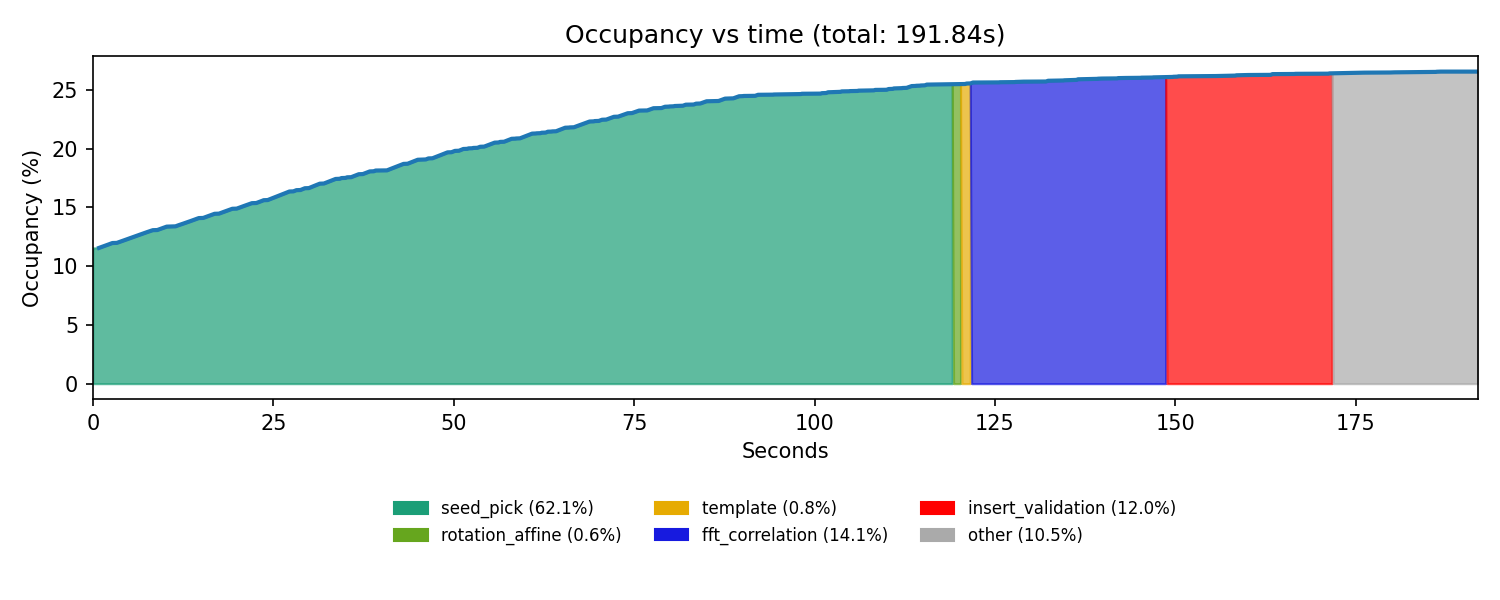
\includegraphics[width=1\textwidth]{archivos/profile_occupancy_breakdown-cpu.png}
        \caption{Tiempo de ejecución en CPU por etapa del algoritmo Tetris. El área coloreada
        bajo la curva de ocupancia indica el tiempo acumulado de cada operación.}
        \label{fig:profile-breakdown}
    \end{figure}
    
    Los resultados, resumidos en la Tabla~\ref{tab:profile}, revelan que \texttt{pick\_seed}
    es el componente de mayor carga computacional, representando el \textbf{62.1\%} del tiempo
    total (119.10\,s). A continuación se sitúan la correlación FFT~3D con un \textbf{14.1\%}
    (27.06\,s) y la validación e inserción con un \textbf{12.0\%} (23.02\,s). El
    \textbf{10.5\%} restante corresponde a operaciones misceláneas de Python e I/O. Las
    operaciones de generación de \textit{in-shell} y rotación afín resultan prácticamente
    despreciables ($<2\%$ combinadas).
    
    \begin{table}[H]
    \centering
    \begin{tabular}{|l|r|r|}
    \hline
    \textbf{Operación} & \textbf{Tiempo (s)} & \textbf{Porcentaje} \\
    \hline
    Selección de semilla (\texttt{pick\_seed}) & 119.10 & 62.1\% \\
    Correlación FFT 3D                         &  27.06 & 14.1\% \\
    Validación e inserción                     &  23.02 & 12.0\% \\
    Otros (Python, I/O)                        &  20.06 & 10.5\% \\
    Generación \textit{in-shell}               &   1.48 &  0.8\% \\
    Rotación afín                              &   1.12 &  0.6\% \\
    \hline
    \textbf{Total}                             & \textbf{191.84} & \textbf{100\%} \\
    \hline
    \end{tabular}
    \caption{Desglose del tiempo de ejecución en CPU de cada operación durante la inserción Tetris.}
    \label{tab:profile}
    \end{table}
    
    Estos datos orientan la estrategia de optimización en dos direcciones: (1)~la aceleración
    GPU reduce el coste de la correlación FFT y la validación mediante paralelismo masivo;
    (2)~la función \texttt{pick\_seed} se beneficia igualmente del backend \texttt{CuPy},
    que ejecuta el \texttt{argwhere} sobre el volumen completo en paralelo, eliminando el
    principal cuello de botella identificado.

    \item \textbf{Esquema final:} Finalmente el algoritmo Tetris queda modificado de la siguiente forma:

    \begin{figure}[H]
        \centering
        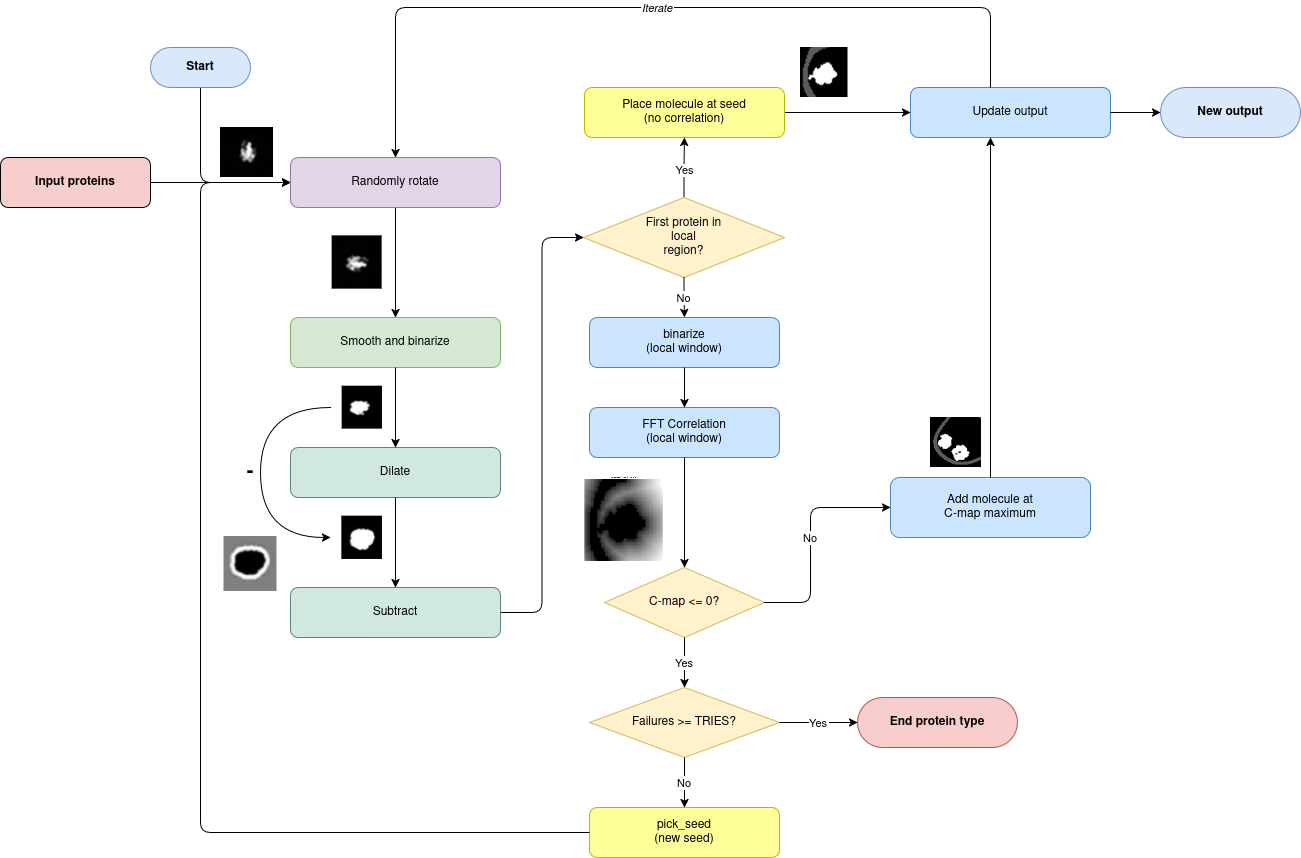
\includegraphics[width=0.7\textwidth]{archivos/tetris-new.png}
        \caption{Diagrama de flujo del algoritmo Tetris modificado.}
        \label{fig:tetris-new}
    \end{figure}
    
    El diagrama ilustra el flujo completo del algoritmo de inserción de proteínas Tetris. A partir de las proteínas de entrada, cada iteración comienza con una rotación aleatoria del volumen molecular, seguida de un suavizado y binarización para obtener una representación binaria de la molécula. A continuación, se generan dos dilataciones del volumen binarizado (exterior e interior) y se restan para construir el \textit{in-shell template}, que codifica la superficie de la proteína con valores positivos en el shell y penalización negativa en el núcleo.
    
    La inserción se delega a \texttt{insert\_molecule\_3d}, que extrae una ventana local alrededor del \textit{seed} seleccionado por \texttt{pick\_seed}. Si la región local está completamente vacía (primera proteína en esa zona) y hay espacio para ella, la molécula se coloca directamente en el \textit{seed} sin necesidad de correlación. En caso contrario, se binariza la ventana local y se realiza una correlación FFT entre dicha ventana y el \textit{in-shell template}, obteniendo un mapa de correlación (C-map) que indica la traslación óptima para empaquetar la nueva proteína junto a las existentes. Si el máximo del C-map es negativo (ninguna posición válida disponible), se incrementa el contador de fallos; al alcanzar el límite \texttt{$T_{cluster}$}, se da por finalizada la inserción del tipo proteico actual. De lo contrario, se selecciona un nuevo \textit{seed} y se reitera el proceso. Tras una inserción exitosa, el volumen de salida se actualiza y el algoritmo itera desde la nueva posición.
    
    
\end{enumerate}

\subsection{Fase 4: Optimización mediante aceleración GPU}

Una vez verificada la corrección lógica de la implementación adaptada, se procedió a su optimización mediante computación paralela en GPU.

\begin{enumerate}
      \item \textbf{Identificación de operaciones paralelizables}: Las dos operaciones más costosas del algoritmo (como se observó antes) son \texttt{insert\_molecule\_3d} —método integrado que engloba la correlación FFT 3D y la validación de inserción, representando conjuntamente el 26.1\% del tiempo total— y \texttt{pick\_seed}, con un 62.1\%, cuyo \texttt{argwhere} sobre el volumen completo se beneficia directamente del paralelismo masivo de la GPU. Ambas operaciones cuentan con implementaciones optimizadas en \texttt{CuPy}. Las operaciones de rotación afín y filtrado gaussiano son computacionalmente despreciables ($<2\%$) pero también se redirigen al backend GPU para mantener los datos en memoria de dispositivo y evitar transferencias innecesarias.

    \item \textbf{Implementación de rutas duales CPU/GPU}: Se implementó un sistema de selección de backend controlado por el flag \texttt{USE\_GPU}. Si \texttt{USE\_GPU = True}, las operaciones se redirigen a las funciones equivalentes de \texttt{cupyx.scipy}; en caso contrario, el código funciona de forma transparente con \texttt{scipy} en CPU, sin cambios en la lógica algorítmica. La Figura~\ref{fig:esquema-gpu-cpu} ilustra este esquema de enrutamiento.


    \begin{figure}[H]
        \centering
        \includegraphics[width=0.65\textwidth]{archivos/esquema_gpu_cpu.png}
        \caption{Esquema de enrutamiento CPU/GPU.}
        \label{fig:esquema-gpu-cpu}
    \end{figure}

    En función de la disponibilidad de una GPU compatible con CUDA, las operaciones de correlación FFT, filtrado gaussiano, rotación afín y muestreo de semilla se ejecutan sobre \texttt{CuPy} (GPU) o \texttt{SciPy/NumPy} (CPU), manteniendo la misma lógica algorítmica en ambos casos.


    \item \textbf{Minimización de transferencias de memoria}: Las transferencias entre memoria principal (CPU) y memoria de la GPU son un cuello de botella conocido en computación heterogénea. Se optimizó el flujo para que cada operación GPU reciba datos NumPy, los convierta a \texttt{cupy.ndarray}, ejecute el cálculo en GPU, y devuelva el resultado de nuevo a NumPy, evitando transferencias intermedias innecesarias.

    \item \textbf{Análisis de rendimiento de la implementación GPU}: Bajo las mismas condiciones experimentales del perfilado CPU (volumen $500\times500\times250$, proteína \textit{2uv8\_10A.pns}, $26.5\%$ de ocupancia), se midió el tiempo de ejecución de la implementación GPU con el mismo script \texttt{profile\_test.py} instrumentado. Los resultados se recogen en la Tabla~\ref{tab:profile-gpu}.

    \begin{table}[H]
    \centering
    \begin{tabular}{|l|r|r|r|r|}
    \hline
    \textbf{Operación} & \textbf{CPU (s)} & \textbf{CPU (\%)} & \textbf{GPU (s)} & \textbf{GPU (\%)} \\
    \hline
    Selección de semilla (\texttt{pick\_seed}) & 119.10 & 62.1\% & 0.54  &  0.7\% \\
    Correlación FFT 3D                         &  27.06 & 14.1\% & 0.62  &  0.8\% \\
    Validación e inserción                     &  23.02 & 12.0\% & 41.36 & 52.3\% \\
    Otros (Python, I/O)                        &  20.06 & 10.5\% & 35.06 & 44.4\% \\
    Generación \textit{in-shell}               &   1.48 &  0.8\% &  1.12 &  1.4\% \\
    Rotación afín                              &   1.12 &  0.6\% &  0.34 &  0.4\% \\
    \hline
    \textbf{Total}                             & \textbf{191.84} & \textbf{100\%} & \textbf{79.04} & \textbf{100\%} \\
    \hline
    \end{tabular}
    \caption{Comparación del desglose de tiempo de ejecución entre las implementaciones CPU y GPU (volumen $500\times500\times250$, proteína \textit{2uv8\_10A.pns}, $26.56\%$ de ocupancia final). La GPU fue una NVIDIA RTX 4090.}
    \label{tab:profile-gpu}
    \end{table}

    La Figura~\ref{fig:profile-breakdown-gpu} muestra la curva de ocupancia frente al tiempo para la ejecución GPU, coloreada por etapa dominante, análoga a la Figura~\ref{fig:profile-breakdown} del perfil CPU.

    \begin{figure}[H]
        \centering
        \includegraphics[width=1\textwidth]{archivos/profile_occupancy_breakdown-gpu.png}
        \caption{Desglose del tiempo de ejecución por etapa de la implementación GPU del algoritmo Tetris. El área coloreada bajo la curva de ocupancia indica el tiempo acumulado de cada operación (experimento: volumen $500\times500\times250$, proteína \textit{2uv8\_10A.pns}, 26.56\% de ocupancia final , NVIDIA RTX 4090).}
        \label{fig:profile-breakdown-gpu}
    \end{figure}

     Los resultados confirman una aceleración global de $\times$\textbf{2.43} (191.84\,s $\to$ 79.04\,s). El beneficio más notable es la eliminación práctica de los dos cuellos de botella originales: \texttt{pick\_seed} pasa de 119.10\,s (62.1\%) a 0.54\,s (0.7\%) gracias al \texttt{argwhere} paralelo de \texttt{CuPy}, y la correlación FFT 3D se reduce de 27.06\,s (14.1\%) a 0.62\,s (0.8\%) mediante \texttt{cupyx.scipy.signal.correlate}. El tiempo restante —validación e inserción (41.36\,s) y otros (35.06\,s)— constituye el piso de tiempo de ejecución inherente al algoritmo: son operaciones de control secuencial, comprobaciones de colisión y gestión del estado interno que no son paralelizables y cuyo coste es equivalente al de la I/O en sistemas convencionales. Este suelo no es reducible mediante aceleración hardware adicional sin un rediseño algorítmico profundo, por lo que la implementación GPU puede considerarse próxima al límite de rendimiento alcanzable con la arquitectura actual.
    
    
\end{enumerate}

\subsection{Fase 5: Evaluación experimental comparativa}

Esta fase cierra la metodología y da paso al Capítulo de Resultados. El objetivo es comparar cuantitativamente Tetris frente a SAWLC bajo las mismas condiciones experimentales. Todos los experimentos utilizan el mismo conjunto de \textbf{11 proteínas solubles} a resolución de 10\,\AA\ (detalladas en el Anexo) y un volumen de membrana real de dimensiones $500\times500\times250$ vóxeles. Las herramientas se organizan en la carpeta \texttt{benchmark/}:

\begin{enumerate}
    \item \textbf{\texttt{profile\_test.py}} — Perfilado por fases de Tetris (CPU o GPU según \texttt{USE\_GPU}). Instrumenta el algoritmo con temporizadores finos y genera una gráfica de ocupancia vs tiempo coloreada por etapa (selección de semilla, rotación, \textit{in-shell}, correlación FFT, validación). Permite identificar qué operaciones dominan el tiempo de ejecución.

    \item \textbf{\texttt{profile\_comparison.py}} — Curva de ocupancia acumulada de los tres algoritmos (Tetris CPU, Tetris GPU y SAWLC) ejecutados secuencialmente sobre el mismo volumen con las 11 proteínas. Produce una gráfica de líneas y un CSV. El objetivo es comparar la velocidad a la que cada algoritmo llena el volumen disponible.

    \item \textbf{\texttt{benchmark\_scientific\_comparison.py}} — Barrido sistemático de targets de ocupancia del 2.5\% al 70\% en pasos de 2.5\%, ejecutando ambos algoritmos en cada punto con caché JSON. Genera 4 gráficas: ocupancia alcanzada vs objetivo, tiempo de ejecución, throughput, y fallos de SAWLC. Permite caracterizar el rendimiento en todo el espectro de densidad.

    \item \textbf{\texttt{sawlc-cpu-gpu/plot\_comparison.py}} — Genera una figura de 4 paneles a partir de logs reales (una ejecución por número de tipos de proteína activos, de 1 a 11): ocupancia total, tiempo de ejecución, población de monómeros por tipo (barras apiladas) y throughput en función de la diversidad molecular.
\end{enumerate}

Las métricas registradas en todos los experimentos son: tiempo de ejecución ($t$), ocupancia de proteínas ($\rho_{prot}$), ocupancia total ($\rho_{total}$), número de monómeros insertados, throughput (monómeros/minuto) y speedup ($t_{SAWLC}/t_{Tetris}$).\\

Esta metodología de cinco fases permitió: (1) establecer un entorno reproducible, (2) comprender el algoritmo de referencia, (3) adaptarlo al contexto de PolNet, (4) optimizarlo mediante GPU, y (5) validarlo experimentalmente frente a SAWLC.



	%%%%%%%%%%%%%%%%%%%%%%%%%%%%%%%%%%%%%%%%%%%%%%%%%%%%%%%%%%%%%%%%%%%%%%%%
% Plantilla TFG/TFM
% Universidad de Murcia. Facultad de Informática
% Realizado por: José Manuel Requena Plens
% Modificado: Pablo José Rocamora Zamora
% Contacto: pablojoserocamora@gmail.com
%%%%%%%%%%%%%%%%%%%%%%%%%%%%%%%%%%%%%%%%%%%%%%%%%%%%%%%%%%%%%%%%%%%%%%%%


\chapter{Resultados}

\section{Curva de ocupancia acumulada con proteína única}

El primer experimento mide exclusivamente la fase de inserción de proteínas, aislando el rendimiento del
algoritmo del resto de la cadena de PolNet. Se utiliza un único tipo de proteína (\texttt{2uv8\_10A},
dimensiones $48 \times 48 \times 48$ vóxeles) sobre el Tomograma 3, cuya membrana pre-existente ocupa
el $11.54\%$ del volumen. Los tres algoritmos (Tetris CPU, Tetris GPU y SAWLC) se ejecutan
secuencialmente sobre el mismo volumen y se registra la ocupancia total acumulada en función del tiempo
transcurrido.

\begin{figure}[H]
    \centering
    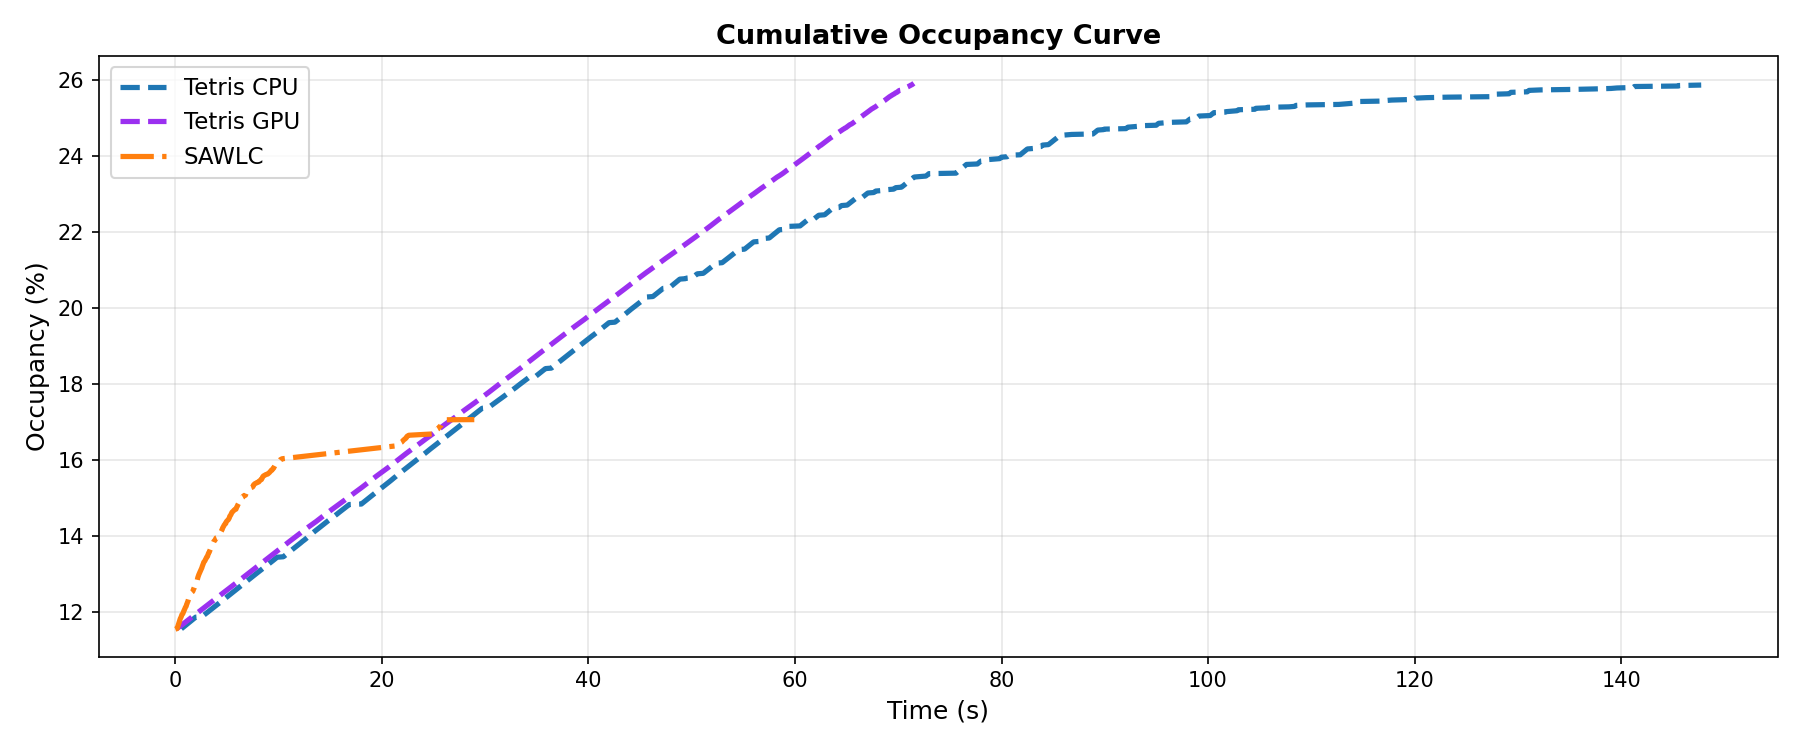
\includegraphics[width=1\textwidth]{archivos/profile_comparison-en.png}
    \caption{Curva de ocupancia acumulada en función del tiempo para los tres algoritmos evaluados
             sobre el Tomograma 3 con la proteína \texttt{2uv8\_10A}. El eje vertical parte del
             $11.5\%$ de la membrana; el incremento posterior corresponde íntegramente a proteínas
             insertadas.}
    \label{fig:profile-comparison}
\end{figure}

La Figura~\ref{fig:profile-comparison} muestra los resultados obtenidos. El eje Y parte del $\approx 11.5\%$
de ocupancia de la membrana, de modo que todo incremento posterior corresponde a proteínas insertadas.
Los resultados ponen de manifiesto tres comportamientos claramente diferenciados:

\begin{itemize}
    \item \textbf{SAWLC} (naranja) finaliza su ejecución en aproximadamente $25$\,s alcanzando una
    ocupancia total de $\approx 16.5\%$, lo que representa en torno a $5$ puntos porcentuales de
    proteína sobre la membrana. La detención temprana se debe a la fragmentación progresiva del espacio
    libre: la caminata aleatoria de SAWLC genera huecos intersticiales demasiado estrechos para alojar
    nuevos monómeros, por lo que el algoritmo agota sus intentos y se termina antes de saturar el volumen.

    \item \textbf{Tetris GPU} (morado) alcanza una ocupancia final de $\approx 25.8\%$ en $\approx 70$\,s.
    La guía por correlación FFT permite al algoritmo identificar y ocupar posiciones de contacto óptimas
    en el espacio libre residual, logrando una densidad de empaquetamiento casi tres veces superior a la
    de SAWLC.

    \item \textbf{Tetris CPU} (azul) converge al mismo techo de ocupancia ($\approx 25.8\%$) que la
    variante GPU pero requiere $\approx 145$\,s, lo que corresponde a un \textit{speedup} de $\approx
    \times 2.1$ del GPU sobre el CPU en este experimento de proteína única.
\end{itemize}

Estos resultados confirman que la estrategia de colocación guiada por FFT de Tetris es capaz de llenar
el volumen de forma significativamente más densa que SAWLC, y que la aceleración GPU reduce el tiempo de
ejecución sin alterar la ocupancia final alcanzada.

\section{Comparativa sistemática en el espectro completo de densidad}

El segundo experimento evalúa ambos algoritmos (Tetris en su variante GPU) a lo largo de un rango amplio
de densidades objetivo. Se define un barrido de \textit{targets} de ocupancia desde el $2.5\%$ hasta el
$57.5\%$ en pasos de $2.5\%$, lo que produce $23$ puntos de evaluación. Para obtener estimaciones
estadísticamente fiables, cada punto se repite \textbf{4 veces}, de modo que las curvas muestran la
media y la desviación típica de las ejecuciones. El experimento utiliza las 11 proteínas del conjunto de
pruebas sobre un tomograma vacío de $500 \times 500 \times 250$ vóxeles.

\begin{figure}[H]
    \centering
    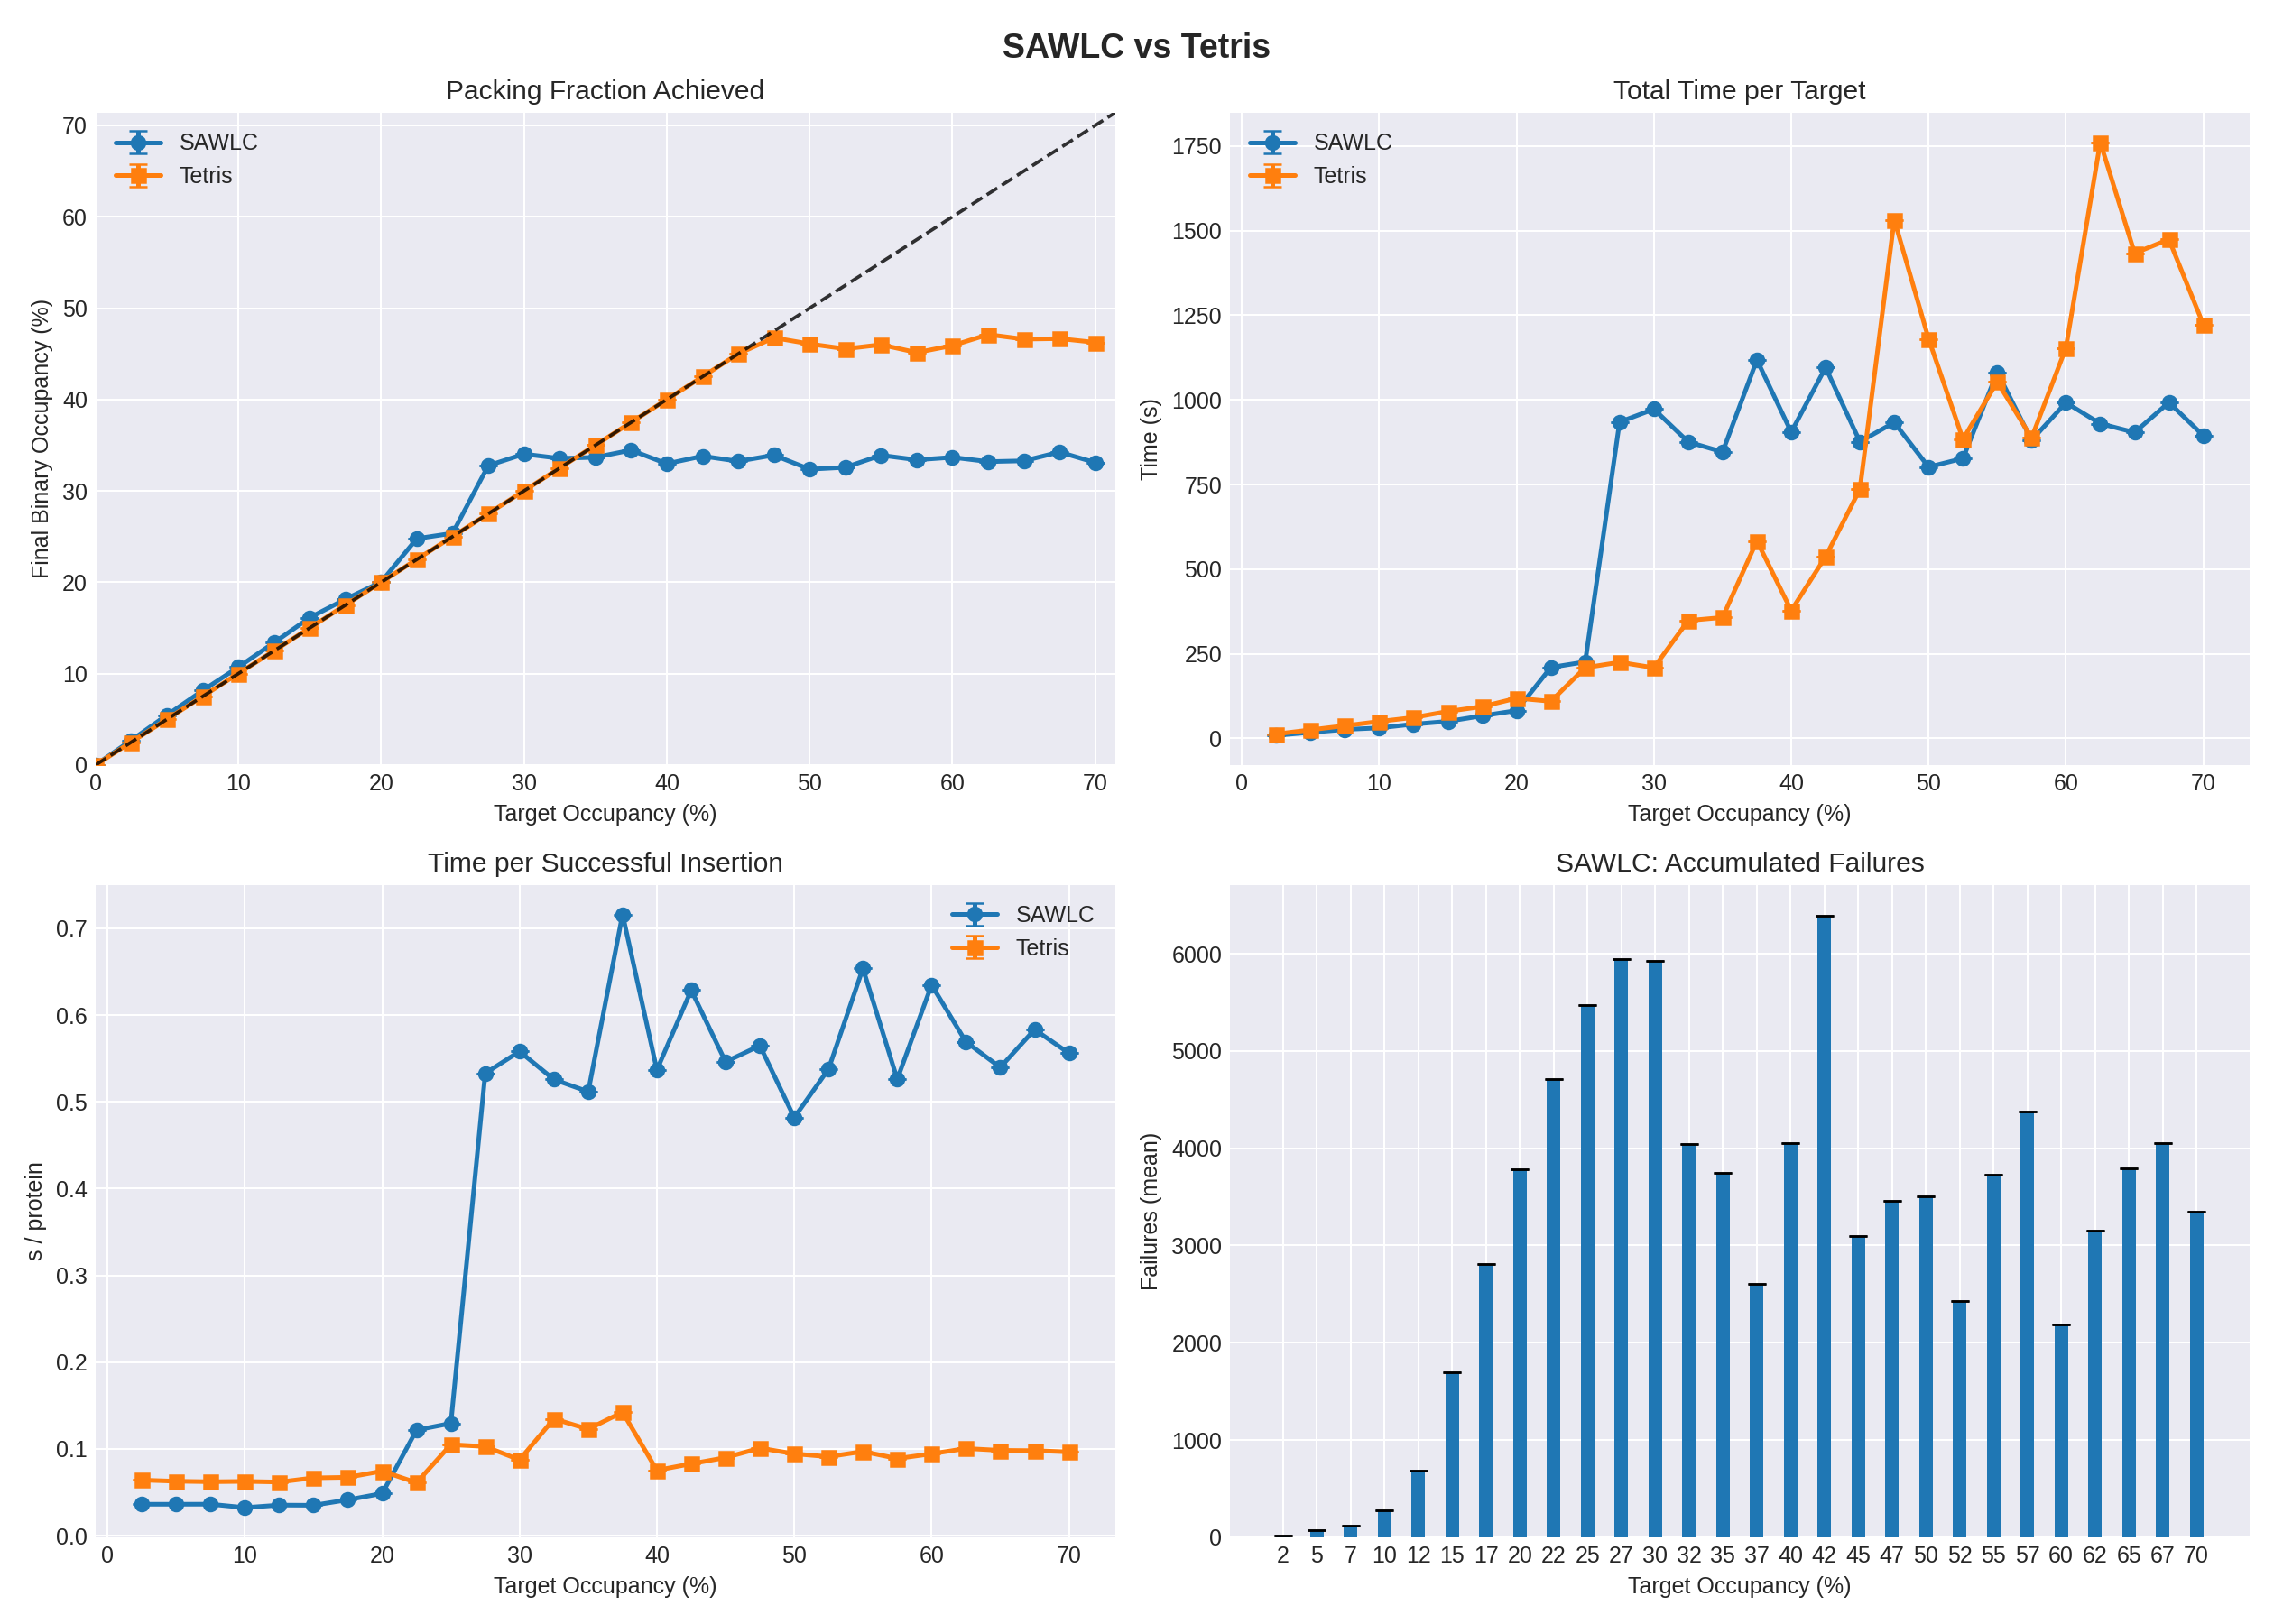
\includegraphics[width=1\textwidth]{archivos/benchmark_scientific_plots.png}
    \caption{Comparativa de ocupancia Tetris y SAWLC a lo largo del espectro completo de densidades
             objetivo. Cada punto representa la media de 4 repeticiones independientes con las 11
             proteínas del conjunto de pruebas.}
    \label{fig:benchmark-scientific}
\end{figure}

La Figura~\ref{fig:benchmark-scientific} agrupa cuatro subgráficas que analizan aspectos complementarios
del rendimiento de ambos algoritmos:

\begin{itemize}
    \item \textbf{Packing Fraction Achieved} (arriba izquierda). Representa la ocupancia final
    obtenida en función del target solicitado. La línea diagonal discontinua marca el ideal de ocupancia
    perfecta ($\text{obtenido} = \text{target}$); cuanto más se acerque una curva a esa diagonal, mayor
    es la capacidad del algoritmo de cumplir el objetivo de densidad.

    \item \textbf{Total Time per Target} (arriba derecha). Muestra el tiempo total de ejecución en
    segundos necesario para que cada algoritmo alcance (o intente alcanzar) el target indicado. Permite
    caracterizar el coste temporal de ambos algoritmos en función de la densidad solicitada.

    \item \textbf{Time per Successful Insertion} (abajo izquierda). Recoge el tiempo medio invertido
    por el algoritmo en insertar un único monómero con éxito, en segundos por proteína. Esta métrica
    refleja la eficiencia intrínseca de cada paso de inserción independientemente del número total de
    monómeros colocados.

    \item \textbf{SAWLC: Accumulated Failures} (abajo derecha). Muestra el número medio acumulado de
    intentos de inserción fallidos de SAWLC antes de que el algoritmo se detenga. Un fallo ocurre cuando
    una semilla candidata es rechazada por solapamiento o por estar fuera de los límites permitidos. Esta
    subgráfica se presenta únicamente para SAWLC porque Tetris, pese a disponer también de un parámetro
    de control de fallos consecutivos (\texttt{TRIES\_CLUSTERING}, con un umbral de 10 intentos), este
    número de fallos no se compara con el que produce SAWLC.
\end{itemize}

\section{Ocupancia máxima en función de la diversidad molecular}

El tercer experimento evalúa cómo evoluciona la ocupancia máxima alcanzable a medida que se incorporan
progresivamente más tipos de proteína. Se diseñan 11 pruebas acumulativas: la primera emplea únicamente
la proteína más grande del conjunto (\texttt{2uv8}), la segunda añade la siguiente en tamaño
(\texttt{5mrc}), y así sucesivamente hasta la prueba 11, en la que se utilizan los 11 tipos de proteína
simultáneamente. En cada prueba los algoritmos corren hasta agotar el volumen disponible sin imponer
ningún target de ocupancia. El tomograma de referencia contiene una membrana pre-existente que ocupa el
$11.5\%$ del volumen (línea discontinua en la Figura~\ref{fig:comparativa-completa}).

\begin{figure}[H]
    \centering
    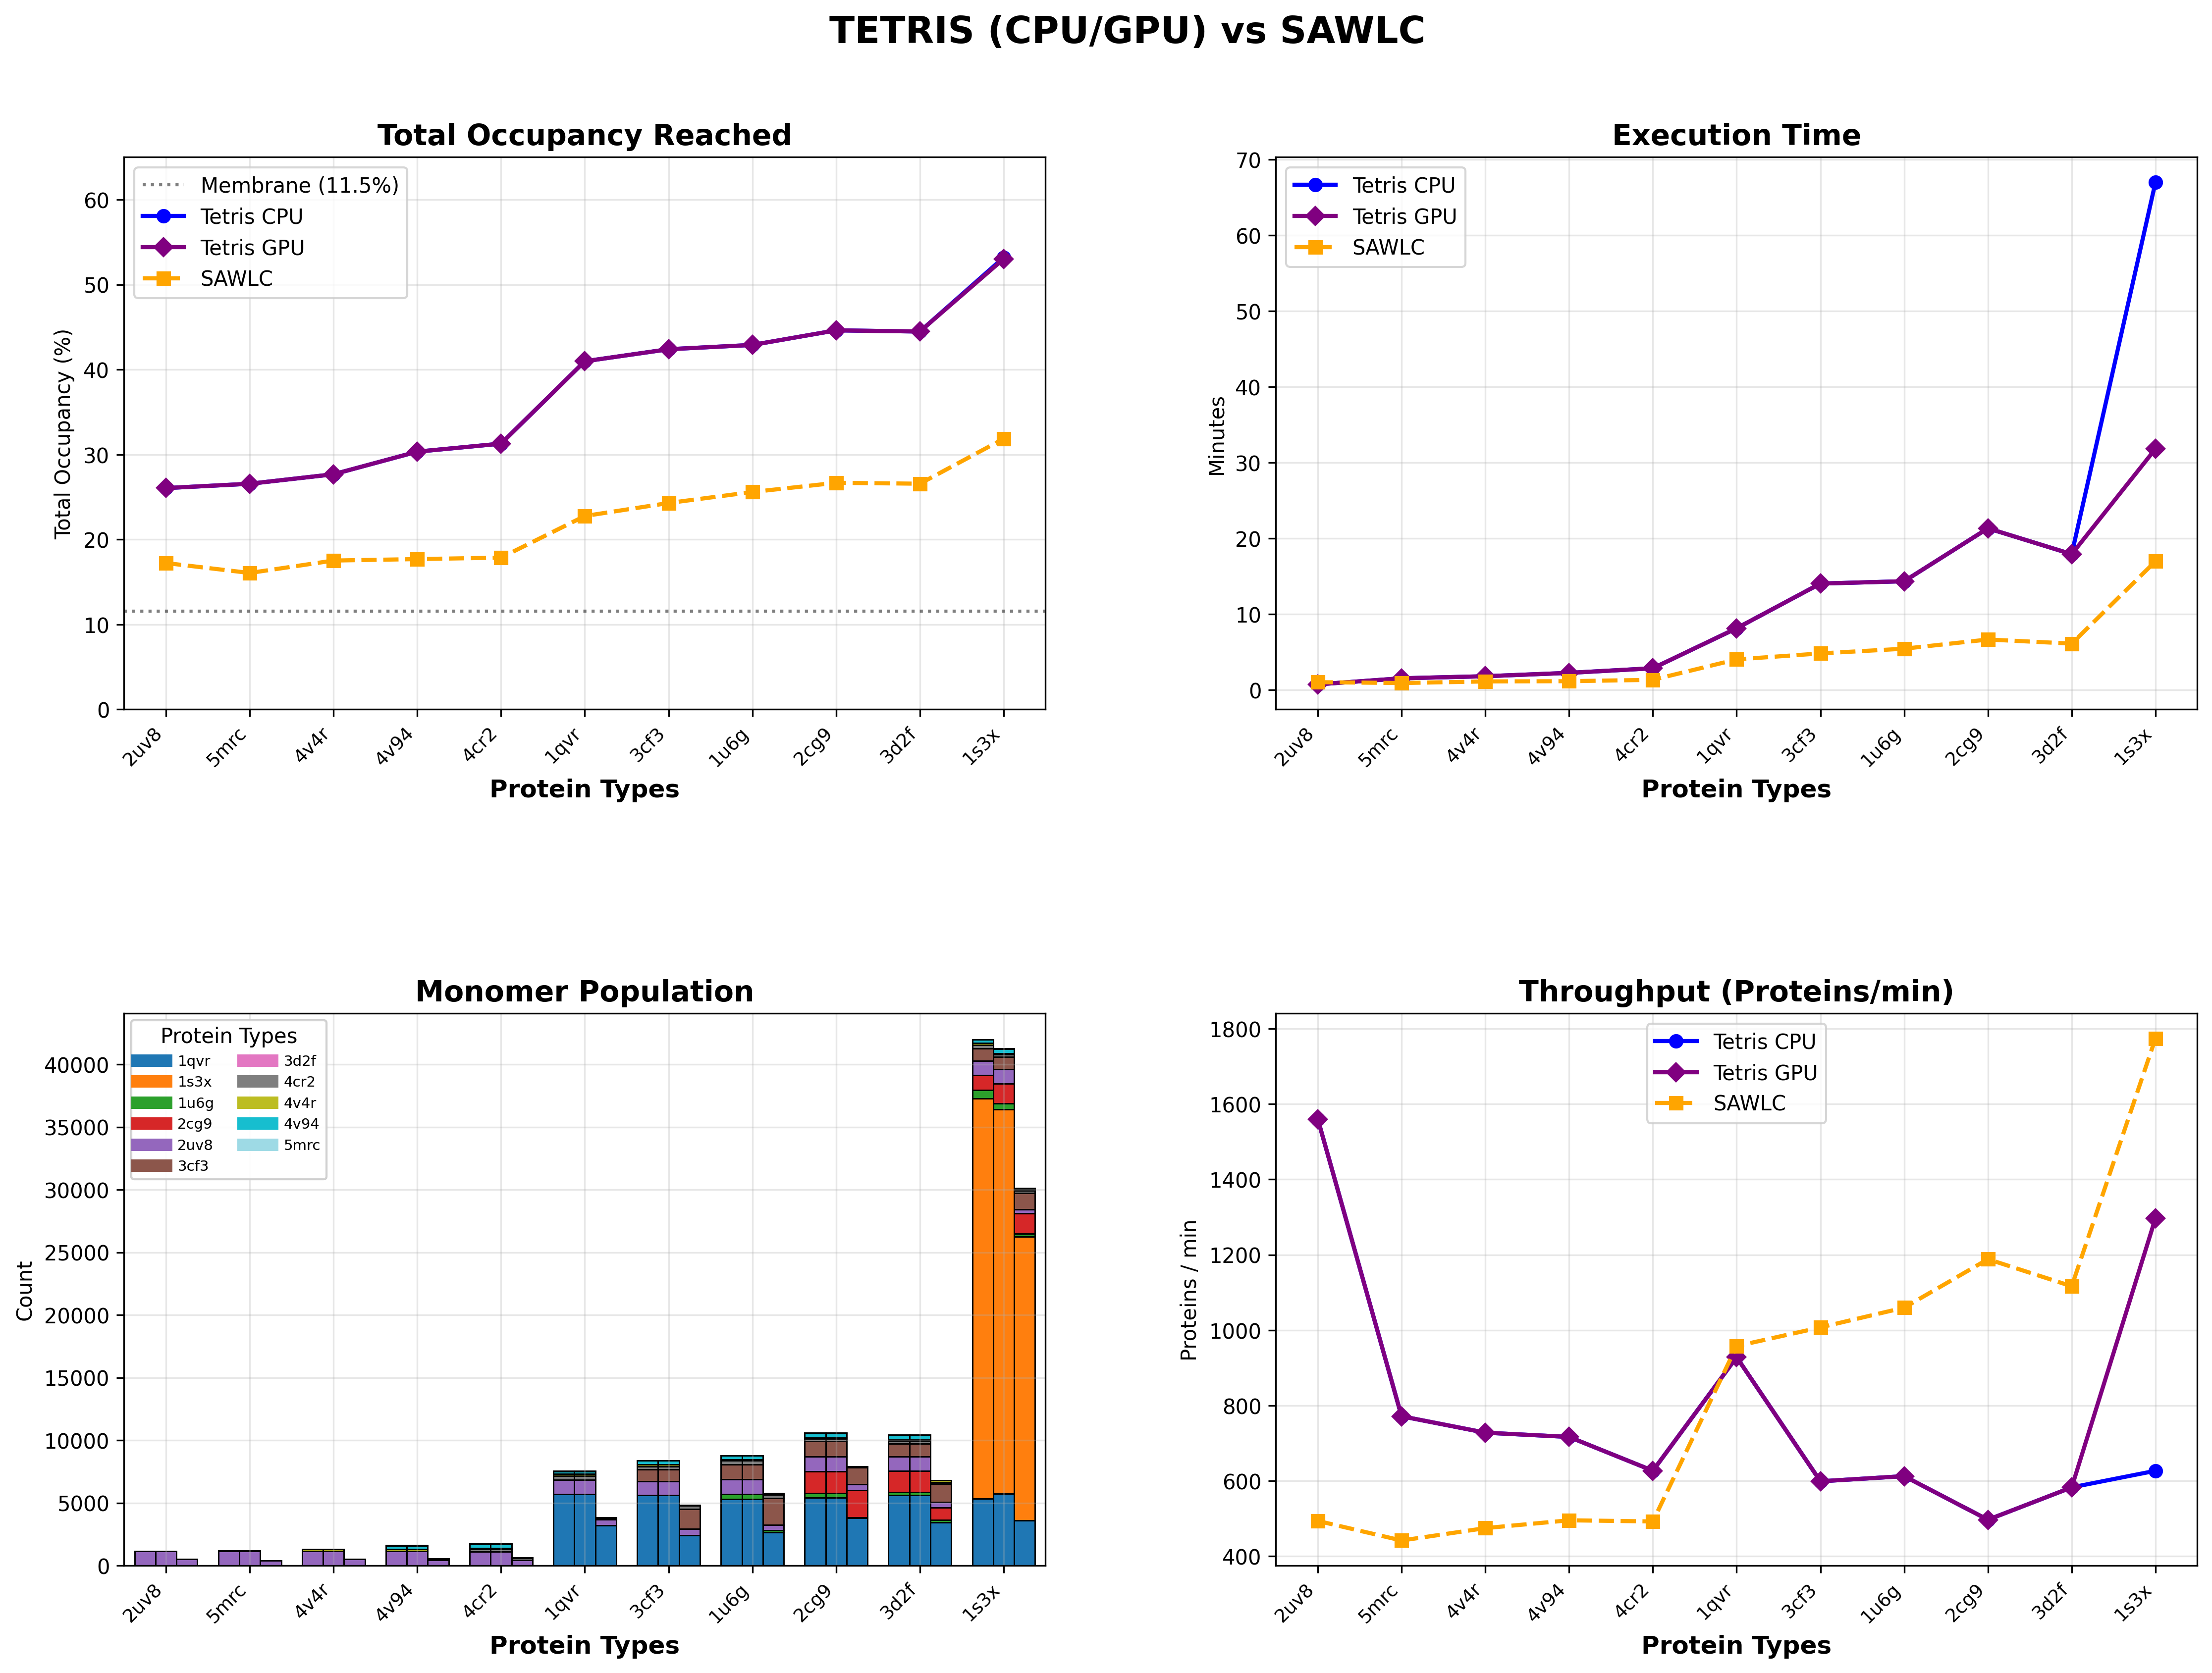
\includegraphics[width=1\textwidth]{archivos/resultados_comparativa_completa.png}
    \caption{Comparativa de Tetris (CPU/GPU) y SAWLC en función del número de tipos de proteína activos.
             Cada punto corresponde a una ejecución hasta saturación sobre el Tomograma 3.}
    \label{fig:comparativa-completa}
\end{figure}

Los resultados de la Figura~\ref{fig:comparativa-completa} muestran un patrón consistente a lo largo
de las cuatro subgráficas. En términos de ocupancia total alcanzada, SAWLC es el algoritmo más rápido
en tiempo de ejecución pero el que menor densidad de empaquetamiento consigue: su caminata aleatoria
satura pronto y deja una fracción significativa del volumen libre sin explotar. Tetris, en cambio,
aprovecha esa capacidad residual gracias a la guía por correlación FFT, lo que se traduce en una
ocupancia total notablemente superior en todas las combinaciones de proteínas. La variante GPU de Tetris
destaca especialmente: con los 11 tipos de proteína activos alcanza una ocupancia total de
aproximadamente el $52\%$ en torno a media hora de ejecución, lo que la convierte en la opción más
equilibrada entre densidad y coste temporal. La variante CPU logra valores de ocupancia similares a los
de la GPU, aunque con tiempos de ejecución sensiblemente mayores.

En cuanto a la población de monómeros, las barras apiladas reflejan que la mayor parte de las
inserciones corresponde a las proteínas de menor tamaño: al ocupar menos volumen individualmente,
pueden llenar los huecos intersticiales que las proteínas grandes dejan libres, contribuyendo de forma
decisiva al incremento de ocupancia total. Finalmente, el panel de throughput muestra que Tetris GPU
mantiene el mayor rendimiento sostenido a lo largo del experimento. SAWLC, por su parte, presenta un
throughput moderado en las primeras pruebas pero registra un pico muy pronunciado al incorporar
\texttt{1s3x}: al poder insertar miles de monómeros diminutos con gran rapidez mediante su caminata
aleatoria, supera puntualmente a Tetris GPU en este último punto. Tetris CPU mantiene el throughput más
bajo de los tres algoritmos de forma consistente.
	%%%%%%%%%%%%%%%%%%%%%%%%%%%%%%%%%%%%%%%%%%%%%%%%%%%%%%%%%%%%%%%%%%%%%%%%
% Plantilla TFG/TFM
% Universidad de Murcia. Facultad de Informática
% Realizado por: José Manuel Requena Plens
% Modificado: Pablo José Rocamora Zamora
% Contacto: pablojoserocamora@gmail.com
%%%%%%%%%%%%%%%%%%%%%%%%%%%%%%%%%%%%%%%%%%%%%%%%%%%%%%%%%%%%%%%%%%%%%%%%


\chapter{Conclusiones y vías futuras}

Este Trabajo Fin de Grado ha abordado el cuello de botella que el algoritmo \textbf{SAWLC} supone en la generación de tomogramas sintéticos dentro de \textbf{PolNet}, adaptando e implementando \textbf{Tetris} como alternativa basada en correlación cruzada 3D mediante FFT. Sobre el algoritmo original se han añadido los mecanismos necesarios para tener en cuenta las estructuras biológicas preexistentes, muestrear semillas válidas en todo el volumen libre y guiar el crecimiento por clústeres compactos. Adicionalmente se ha desarrollado una versión acelerada por GPU y un banco de pruebas reproducible que compara Tetris CPU, Tetris GPU y SAWLC bajo las mismas condiciones experimentales.\\

La aportación conceptual principal es la \textbf{reformulación de la inserción de proteínas como un problema de optimización global discreta}. Mientras SAWLC plantea la colocación como un proceso estocástico de prueba-y-error cuyo coste crece de forma no lineal con la densidad del volumen, Tetris la formula como la búsqueda del máximo de un mapa de correlación calculado en $O(V \log V)$ por inserción, independientemente del grado de saturación. Los resultados experimentales muestran que Tetris alcanza grados de ocupancia claramente mayores que SAWLC, lo que permite ampliar la escala y la densidad de los conjuntos de datos sintéticos empleados en el entrenamiento de redes neuronales profundas para tareas de segmentación, \textit{particle picking} y \textit{denoising}.\\

La línea de continuación natural y prioritaria del proyecto es la \textbf{integración definitiva de Tetris dentro del \textit{framework} PolNet} como módulo de inserción. Adicionalmente, sería interesante extender el algoritmo más allá de las proteínas solubles para que pueda manejar también otros elementos biológicos del tomograma, como filamentos o proteínas de membrana, lo que requeriría adaptar la construcción del \textit{in-shell template} para incorporar restricciones direccionales y de anclaje a superficie.

	%\input{capitulos/_introduccion}		% Plantilla: Se muestran contenidos
	%\input{capitulos/_marcoteorico}		% Plantilla: Se muestran listas
	%\input{capitulos/_objetivos}		% Plantilla: Se muestran tablas
	%\input{capitulos/_metodologia}		% Plantilla: Se muestran figuras
	%\input{capitulos/_desarrollo}		% Plantilla: Se muestran listados
	%\input{capitulos/_resultados}		% Plantilla: Se muestran gráficas
	%\input{capitulos/_conclusiones}		% Plantilla: Se muestran matemáticas
	
	%%%%
	% CONTENIDO. BIBLIOGRAFÍA.
	%%%%
	\nocite{*} %incluye TODOS los documentos de la base de datos bibliográfica sean o no citados en el texto
	\bibliographystyle{unsrtnat}
	\bibliography{bibliografia/bibliografia} % Archivo que contiene la bibliografía
	
	
	%%%%
	% CONTENIDO. LISTA DE ACRÓNIMOS. Comenta las líneas si no lo deseas incluir.
	%%%%
	% Incluye el listado de acrónimos utilizados en el trabajo. 
	% printglossary[style=modsuper,type=\acronymtype,title={Lista de Acrónimos y Abreviaturas}]
	% Añade el resto de acrónimos si así se desea. Si no elimina el comando siguiente
	% \glsaddallunused
	
	%%%%
	% CONTENIDO. Anexos - Añade o elimina según tus necesidades
	%%%%
	\appendix % Inicio de los apéndices
	%%%%%%%%%%%%%%%%%%%%%%%%%%%%%%%%%%%%%%%%%%%%%%%%%%%%%%%%%%%%%%%%%%%%%%%%
% Plantilla TFG/TFM
% Universidad de Murcia. Facultad de Informática
% Realizado por: José Manuel Requena Plens
% Modificado: Pablo José Rocamora Zamora
% Contacto: pablojoserocamora@gmail.com
%%%%%%%%%%%%%%%%%%%%%%%%%%%%%%%%%%%%%%%%%%%%%%%%%%%%%%%%%%%%%%%%%%%%%%%%

\chapter{Anexo}

\begin{table}[h]
\centering
\label{tab:proteinas}
\begin{tabular}{lcccc}
\toprule
\textbf{Proteína} & \textbf{Dimensiones} & \textbf{Volumen total} & \textbf{Vóxels ocupados} & \textbf{Ocupancia interna} \\
    \midrule
    4v4r\_10A & $66 \times 66 \times 66$ & 287\,496 & 5\,440 & 1.89\,\% \\
    5mrc\_10A & $72 \times 72 \times 72$ & 373\,248 & 7\,599 & 2.04\,\% \\
    2uv8\_10A & $48 \times 48 \times 48$ & 110\,592 & 7\,458 & 6.74\,\% \\
    4v94\_10A & $72 \times 72 \times 72$ & 373\,248 & 4\,985 & 1.34\,\% \\
    4cr2\_10A & $66 \times 66 \times 66$ & 287\,496 & 3\,499 & 1.22\,\% \\
    3d2f\_10A & $62 \times 62 \times 62$ & 238\,328 &    739 & 0.31\,\% \\
    3cf3\_10A & $54 \times 54 \times 54$ & 157\,464 &    814 & 0.52\,\% \\
    2cg9\_10A & $52 \times 52 \times 52$ & 140\,608 &    576 & 0.41\,\% \\
    1u6g\_10A & $56 \times 56 \times 56$ & 175\,616 &    741 & 0.42\,\% \\
    1s3x\_10A & $46 \times 46 \times 46$ &  97\,336 &    156 & 0.16\,\% \\
    1qvr\_10A & $56 \times 56 \times 56$ & 175\,616 &    957 & 0.54\,\% \\
    \bottomrule
\end{tabular}
\caption{Proteínas utilizadas en los experimentos (resolución 10\,\AA).}
\end{table}


\begin{figure}[H]
    \centering
    \begin{subfigure}[b]{0.36\textwidth}
        \centering
        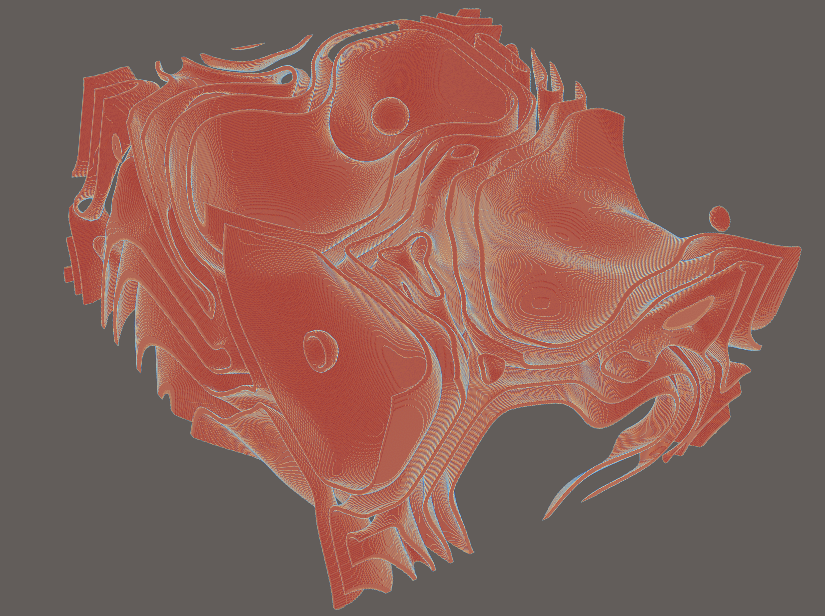
\includegraphics[width=\textwidth]{archivos/membrana0.png}
        \caption{Ocupancia base de 12.88\%}
    \end{subfigure}
     \hspace{0.04\textwidth}
    \begin{subfigure}[b]{0.36\textwidth}
        \centering
        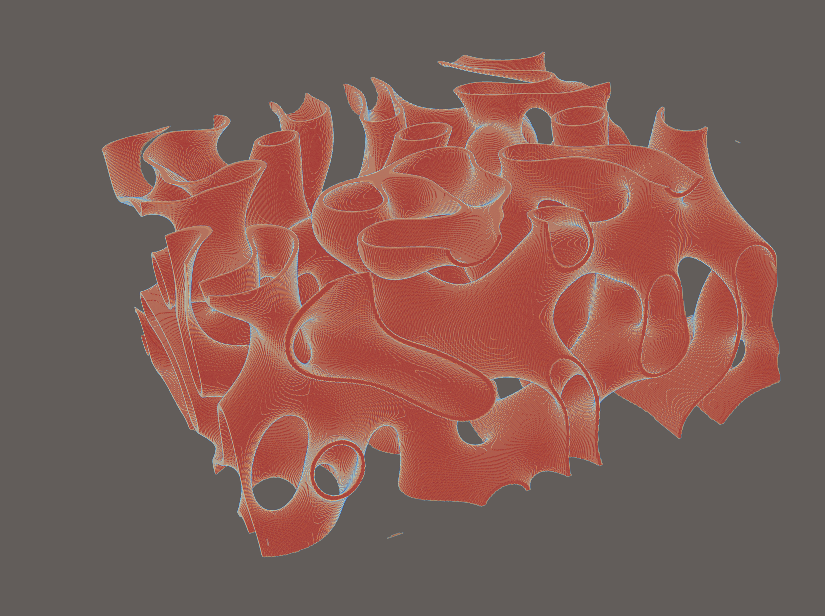
\includegraphics[width=\textwidth]{archivos/membrana1.png}
        \caption{Ocupancia base de 7.43\%}
    \end{subfigure}
    
    \begin{subfigure}[b]{0.36\textwidth}
        \centering
        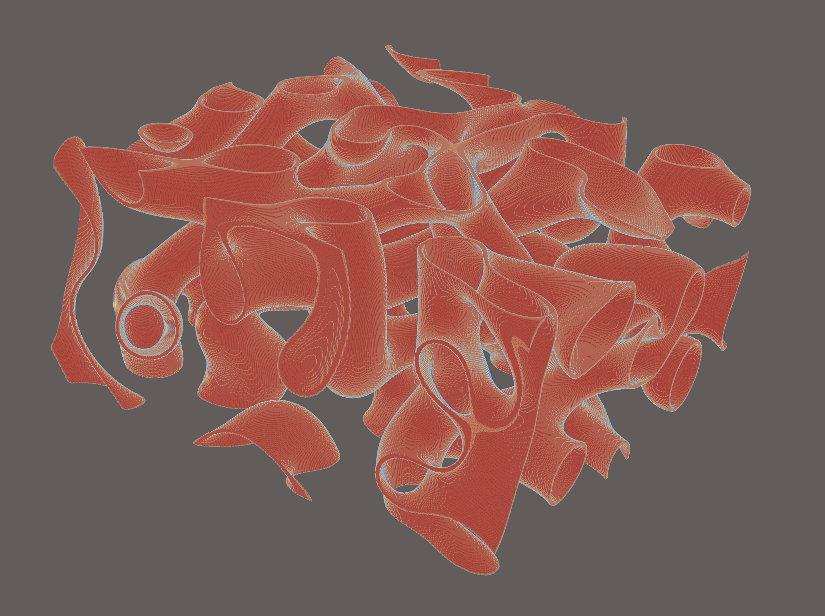
\includegraphics[width=\textwidth]{archivos/membrana2.png}
        \caption{Ocupancia base de 6.63\%}
    \end{subfigure}
     \hspace{0.04\textwidth}
    \begin{subfigure}[b]{0.36\textwidth}
        \centering
        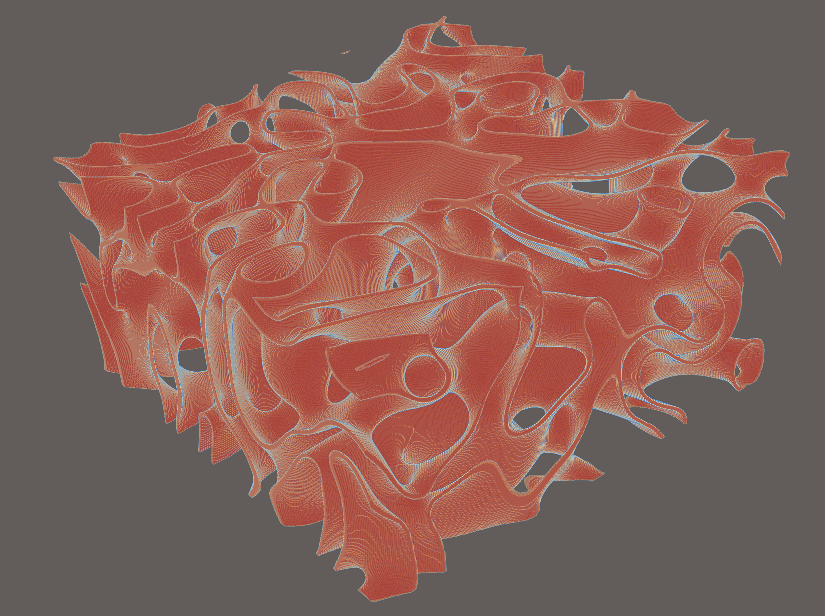
\includegraphics[width=\textwidth]{archivos/membrana3.png}
        \caption{Ocupancia base de 11.54\%}
    \end{subfigure}
    \caption{Membranas sintéticas utilizadas en los experimentos.}
    \label{fig:membranas}
\end{figure}

\begin{figure}[H]
    \centering
    \captionsetup[subfigure]{labelformat=empty}
    \begin{subfigure}[b]{0.36\textwidth}
        \centering
        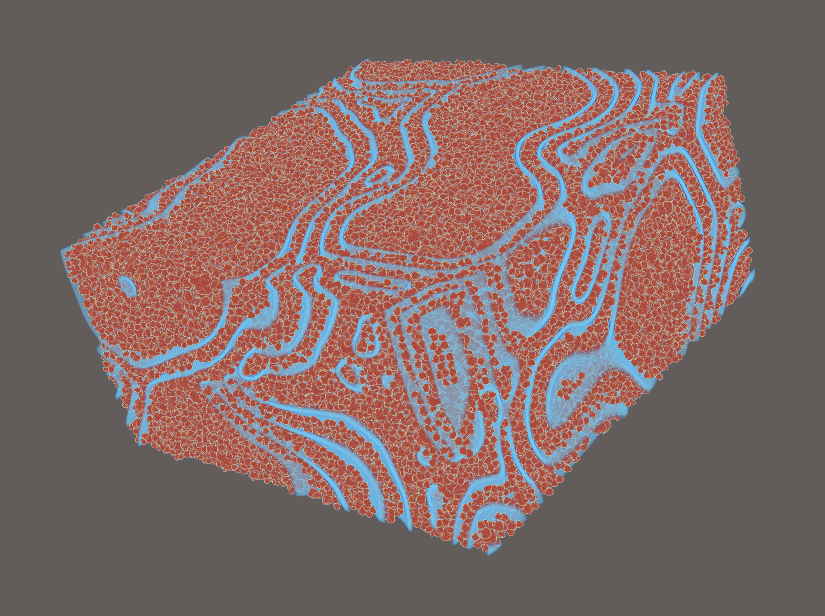
\includegraphics[width=\textwidth]{archivos/tomo0.png}
        \caption{Membrana \textbf{a)}: proteínas 39.25\%, total 52.13\%}
    \end{subfigure}
    \hspace{0.04\textwidth}
    \begin{subfigure}[b]{0.36\textwidth}
        \centering
        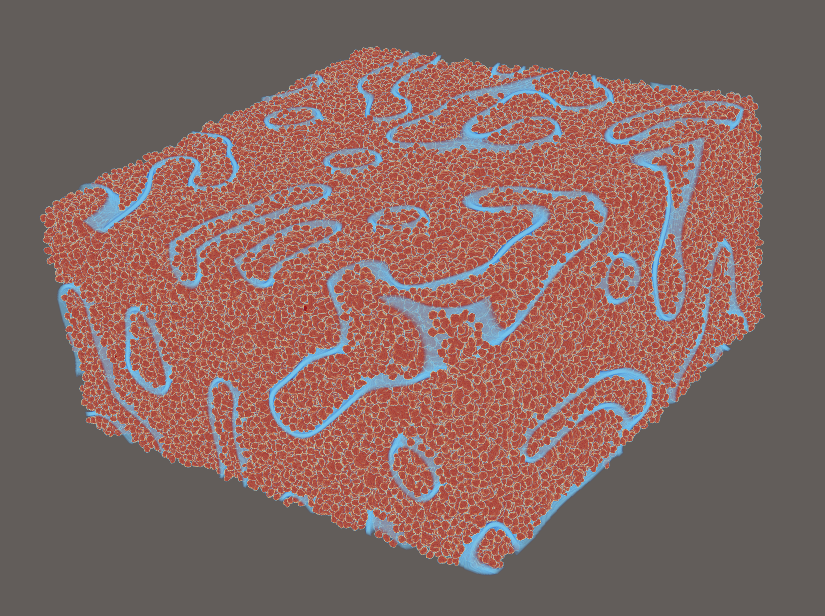
\includegraphics[width=\textwidth]{archivos/tomo1.png}
        \caption{Membrana \textbf{b)}: proteínas 46.55\%, total 53.99\%}
    \end{subfigure}

    \begin{subfigure}[b]{0.36\textwidth}
        \centering
        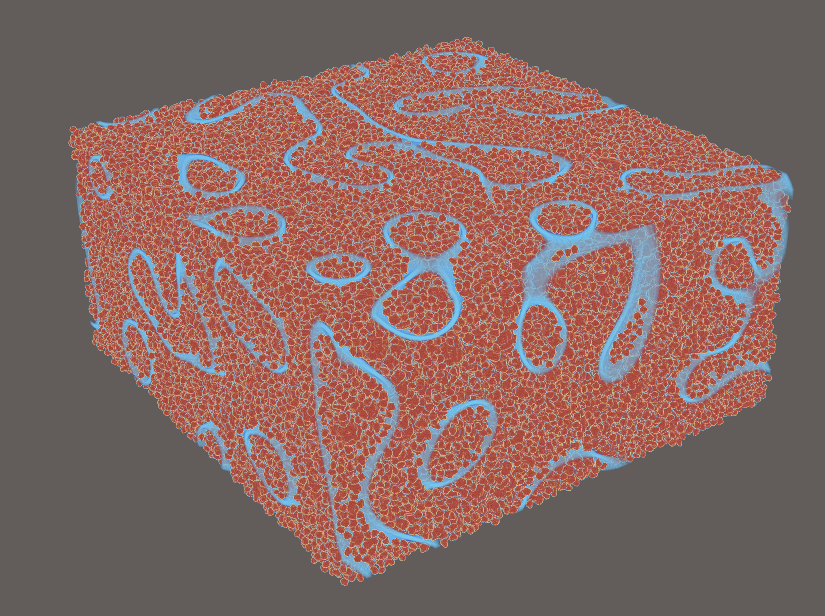
\includegraphics[width=\textwidth]{archivos/tomo2.png}
        \caption{Membrana \textbf{c)}: proteínas 47.62\%, total 54.25\%}
    \end{subfigure}
    \hspace{0.04\textwidth}
    \begin{subfigure}[b]{0.36\textwidth}
        \centering
        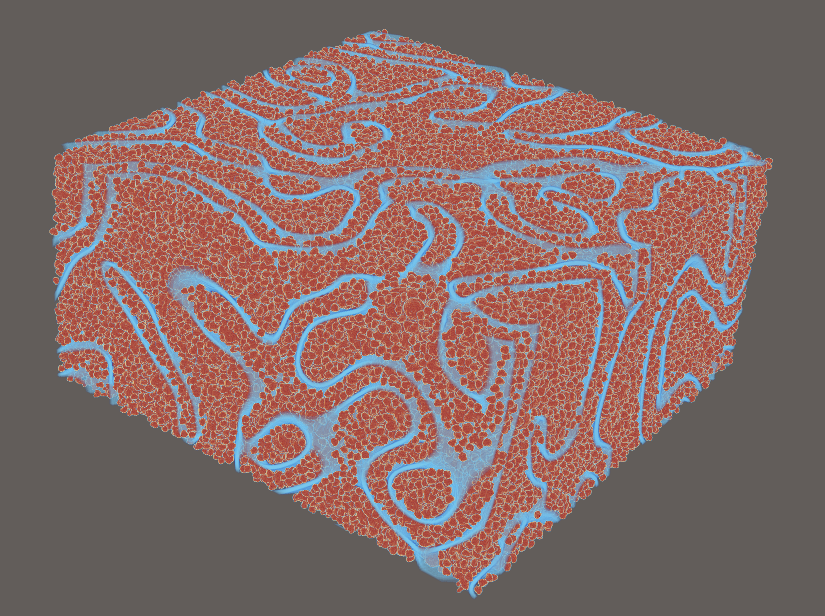
\includegraphics[width=\textwidth]{archivos/tomo3.png}
        \caption{Membrana \textbf{d)}: proteínas 41.65\%, total 53.19\%}
    \end{subfigure}
    \caption{Tomogramas sintéticos generados con Tetris para cada membrana.}
    \label{fig:tomos}
\end{figure}


\begin{table}[h]
\centering
\begin{tabular}{lrrrr}
\toprule
\textbf{Proteína} & \textbf{Membrana a)} & \textbf{Membrana b)} & \textbf{Membrana c)} & \textbf{Membrana d)} \\
\midrule
2uv8\_10A &    777  & 1\,805 & 1\,883 & 1\,140 \\
5mrc\_10A &     52  &    15  &    23  &    44  \\
4v4r\_10A &    155  &   212  &   230  &   137  \\
4v94\_10A &    111  &    98  &    41  &   230  \\
4cr2\_10A &    176  &   324  &   319  &   390  \\
1qvr\_10A &  7\,876 & 3\,981 & 3\,912 & 5\,268 \\
3cf3\_10A &  1\,234 & 1\,078 & 1\,404 & 1\,056 \\
1u6g\_10A &    567  &   635  &   211  &   417  \\
2cg9\_10A &    928  & 1\,428 & 1\,938 & 1\,510 \\
3d2f\_10A &     51  &     0  &     1  &     0  \\
1s3x\_10A & 31\,716 & 29\,812 & 29\,822 & 31\,657 \\
\midrule
\textbf{Total} & \textbf{43\,643} & \textbf{39\,388} & \textbf{39\,784} & \textbf{41\,849} \\
\bottomrule
\end{tabular}
\caption{Número de monómeros insertados por tipo de proteína en cada membrana usando Tetris.}
\label{tab:monomeros}
\end{table}


\begin{figure}[H]
    \centering
    \captionsetup[subfigure]{labelformat=empty}
    \begin{subfigure}[b]{0.36\textwidth}
        \centering
        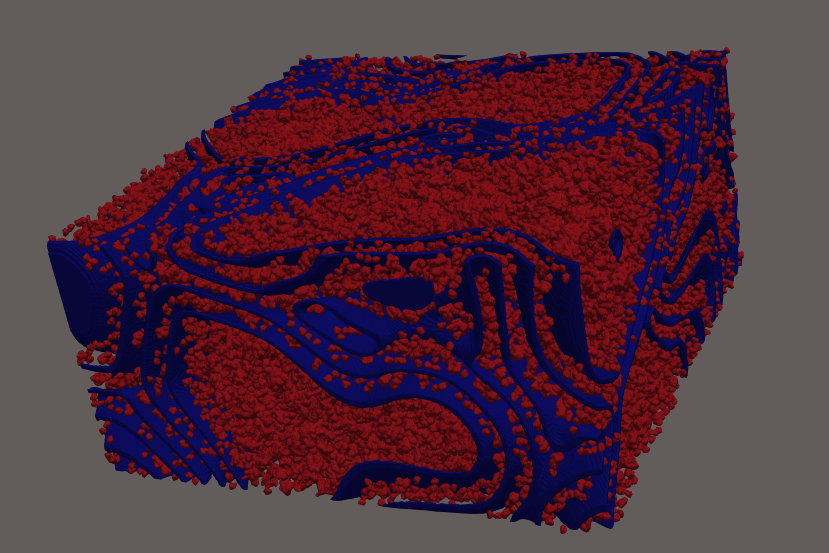
\includegraphics[width=\textwidth]{archivos/tomo_0-sawlc.png}
        \caption{Membrana \textbf{a)}: proteínas 18.63\%, total 31.51\%}
    \end{subfigure}
    \hspace{0.04\textwidth}
    \begin{subfigure}[b]{0.36\textwidth}
        \centering
        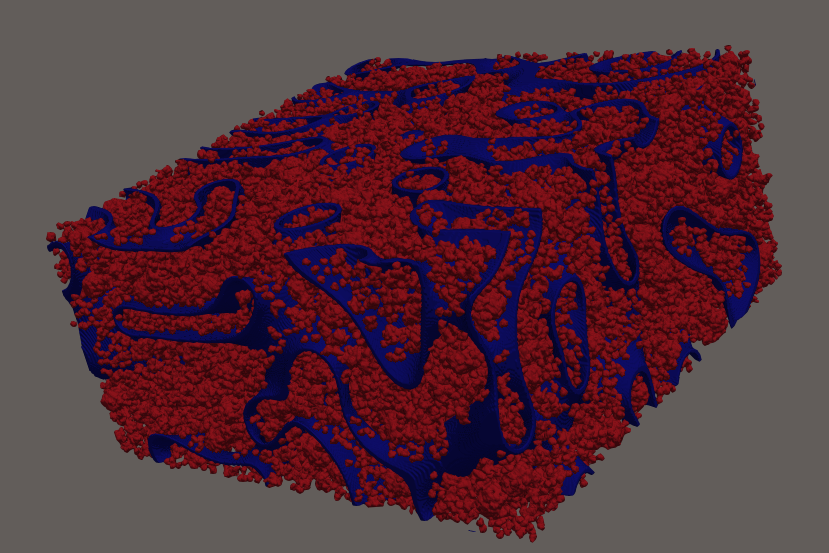
\includegraphics[width=\textwidth]{archivos/tomo_1-sawcl.png}
        \caption{Membrana \textbf{b)}: proteínas 23.66\%, total 31.10\%}
    \end{subfigure}

    \begin{subfigure}[b]{0.36\textwidth}
        \centering
        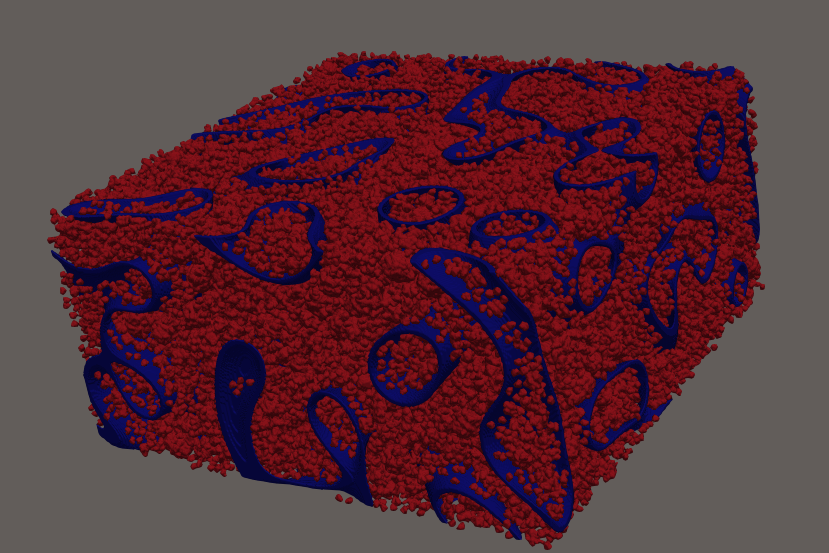
\includegraphics[width=\textwidth]{archivos/tomo_2-sawlc.png}
        \caption{Membrana \textbf{c)}: proteínas 27.08\%, total 33.71\%}
    \end{subfigure}
    \hspace{0.04\textwidth}
    \begin{subfigure}[b]{0.36\textwidth}
        \centering
        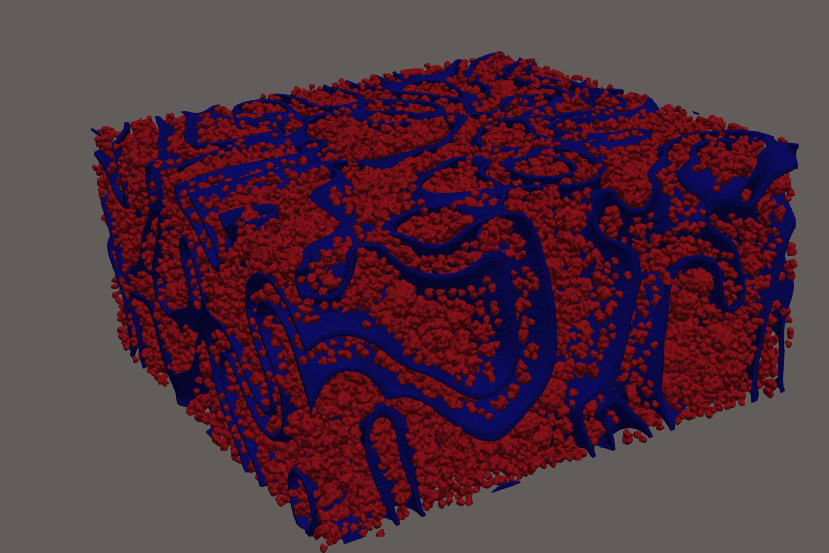
\includegraphics[width=\textwidth]{archivos/tomo_3-sawlc.png}
        \caption{Membrana \textbf{d)}: proteínas 20.17\%, total 31.72\%}
    \end{subfigure}
    \caption{Tomogramas sintéticos generados con SAWLC para cada membrana.}
    \label{fig:tomos-sawlc}
\end{figure}

\begin{table}[h]
\centering
\begin{tabular}{lrrrr}
\toprule
\textbf{Proteína} & \textbf{Membrana a)} & \textbf{Membrana b)} & \textbf{Membrana c)} & \textbf{Membrana d)} \\
\midrule
2uv8\_10A &    362  &    946  & 1\,052 &    446  \\
5mrc\_10A &      3  &      9  &     10 &     14  \\
4v4r\_10A &     45  &     60  &     57 &     86  \\
4v94\_10A &      7  &      0  &     41 &      9  \\
4cr2\_10A &    137  &    168  &     72 &    208  \\
1qvr\_10A &  1\,816 &  2\,836 & 2\,773 &  3\,059 \\
3cf3\_10A &  2\,119 &  1\,103 & 1\,632 &  1\,178 \\
1u6g\_10A &    873  &    287  &    116 &    401  \\
2cg9\_10A &  1\,781 &    409  & 1\,544 &  1\,642 \\
3d2f\_10A &     88  &     20  &     14 &     20  \\
1s3x\_10A & 23\,993 & 23\,159 & 27\,953 & 23\,231 \\
\midrule
\textbf{Total} & \textbf{31\,224} & \textbf{28\,997} & \textbf{35\,264} & \textbf{30\,294} \\
\bottomrule
\end{tabular}
\caption{Número de monómeros insertados por tipo de proteína en cada membrana usando SAWLC.}
\label{tab:monomeros-sawlc}
\end{table}
	% \input{anexos/_anexo_2}
	% \input{anexos/_anexo_3}
	
\end{document}